\documentclass{llncs}

\usepackage{amssymb, amsmath}
\usepackage[utf8]{inputenc}
\usepackage[T1]{fontenc}
\usepackage{unicode}
\usepackage{tikz}
\usepackage{hyperref}
\usepackage{multirow}
\usepackage{bigdelim}
\usepackage[ruled, vlined, linesnumbered]{algorithm2e}
\SetEndCharOfAlgoLine{}
\SetKwInput{Params}{Public parameters}
\SetKwInput{Key}{Shared key}
\SetKwInput{Input}{Input}
\SetKwInput{Output}{Output}
\SetKwBlock{Alice}{Alice}{}
\SetKwBlock{Bob}{Bob}{}
\SetKw{Samples}{samples}
\SetKw{Sends}{sends}
\SetKw{Sends}{sends}
\SetKwProg{Function}{function}{}{}
\SetKwFunction{KeyGen}{KeyGen}
\SetKwFunction{DH}{DH}

%Shortcuts
\newcommand{\F}{\mathbb{F}}
\newcommand{\Fbar}{\overline{\mathbb{F}}}
\newcommand{\Q}{\mathbb{Q}}
\newcommand{\Z}{\mathbb{Z}}
\newcommand{\C}{\mathbb{C}}
\newcommand{\Cl}{\mathcal{C}}
\newcommand{\Graph}{\mathcal{G}}
\renewcommand{\O}{\mathcal{O}}
\newcommand{\softO}{\tilde{O}}
\newcommand{\isom}{\overset{\sim}{\longrightarrow}}
\newcommand{\from}{\ensuremath{\,:\ }}
\newcommand{\set}[1]{\left\{#1\right\}}
\newcommand{\suchthat}{\,\middle\vert\,}
\newcommand{\algstyle}[1]{\textsc{#1}}
\renewcommand{\v}{\vspace{5mm}}
\renewcommand{\frak}{\mathfrak}
\newcommand{\rand}[1]{\overset{#1}{∈}}
\newcommand{\uni}{\rand{R}}
\newcommand{\Adv}[2][]{\mathsf{Adv}^{#1}_{\text{\rm #2}}}

\DeclareMathOperator{\End}{End}
\DeclareMathOperator{\Ker}{Ker}
\DeclareMathOperator{\Card}{Card}
\DeclareMathOperator{\Ell}{Ell}
\DeclareMathOperator{\poly}{poly}
\DeclareMathOperator{\Proba}{Pr}

\begin{document}

\title{Towards practical key exchange from ordinary isogeny graphs}
\author{
  Luca De Feo\inst{1,3}\orcidID{0000-0002-9321-0773} \and
  Jean Kieffer\inst{2} \and
  Benjamin Smith\inst{3}}
\institute{
  Université Paris Saclay, UVSQ, LMV, Versailles, France \and
  École Normale Supérieure, Paris, France \and
  Inria Saclay, Palaiseau, France
}

\maketitle

\begin{abstract}
    We revisit the ordinary isogeny-graph based cryptosystems
    of Couveignes and Rostovtsev--Stolbunov,
    long dismissed as impractical.
    We give algorithmic improvements that accelerate key exchange
    in this framework,
    and explore the problem of generating suitable system parameters
    for contemporary pre- and post-quantum security that take
		advantage of these new algorithms.
    We also prove the session-key security of this key exchange
    in the Canetti--Krawczyk model,
    and the IND-CPA security of the related public-key encryption scheme,
    under reasonable assumptions on the hardness of computing isogeny walks.
    Our systems admit efficient key-validation techniques that
    yield CCA-secure encryption,
    thus providing an important step towards
    efficient post-quantum non-interactive key exchange.

  \keywords{Post-quantum cryptography \and Key exchange \and Elliptic curves \and Isogenies}
\end{abstract}

\section{Introduction}
\label{sec:introduction}

A recent trend in cryptography is the development of quantum-safe
cryptosystems: protocols based on mathematical problems not known to
be solvable in polynomial time by quantum computers. With Shor's
algorithm~\cite{shor1994algorithms} ruling out systems based on
integer factorization or discrete logarithms, NIST has launched a
process to standardize the next generation of \emph{post-quantum}
public key cryptosystems~\cite{NIST2016}. In response, NIST has
received 69 proposals, most of them belonging to the three more
popular post-quantum families: lattice-based systems, code-based
systems, and multivariate systems. Among the youngest and least
explored families, \emph{isogeny-based} cryptography features only one
proposal to the NIST competition: the Supersingular Isogeny Key
Encapsulation (SIKE)~\cite{SIKE}.

SIKE is based upon the key-exchange protocol by Jao and De
Feo~\cite{jao+defeo2011}, known as SIDH, itself inspired by earlier
key-exchange constructions by Couveignes~\cite{cryptoeprint:2006:291}
and Rostovtsev and
Stolbunov~\cite{rostovtsev+stolbunov06,stolbunov-red,Stol}. The
origins of isogeny-based cryptography can be traced back to
Couveignes' seminal work ``Hard Homogeneous Spaces'', that went
unpublished for ten years before appearing
in~\cite{cryptoeprint:2006:291}. 

A \emph{principal homogeneous space} for a group $G$ is a set $X$ with an
action of $G$ on $X$ such that for any $x∈X$ the map $φ_x:g↦g·x$ is an
isomorphism between $G$ and $X$. Intuitively, one can think of $X$ as
a copy (or, rather, many different copies) of $G$ where
the identity element has been forgotten. 

Couveignes defines a \emph{hard homogeneous space} (HHS) 
to be a principal homogeneous space 
where the action of $G$ on $X$ is efficiently computable, 
but inverting the isomorphism $φ_x$ is computationally hard for any $x$.
Algorithm~\ref{alg:HHS-KeyGen} generates private-public keypairs
for cryptosystems based on the hardness of inverting $\varphi_x$.

\begin{algorithm}
    \caption{Key generation for cryptosystems in an HHS $X$ for a
    group $G$, with a fixed ``base point'' $x_0$ in $X$.}
    \label{alg:HHS-KeyGen}
    \KwIn{()}
    \KwOut{A private-public keypair $(g,x)\in G\times X$
    s.t. $x = g\cdot x_0$}
    \Function{\KeyGen{}}{
        $g \gets \algstyle{Random}(G)$
        \tcp*{$\sigma$ is sampled uniformly at random from $G$}
        $x \gets g\cdot x_0$
        \;
        \Return{$(g,x)$}
    }
\end{algorithm}

Any HHS $X$ for an abelian group $G$ can be used to construct a
key exchange as shown in Algorithm~\ref{alg:HHS-DH}.
If Alice and Bob have keypairs $(g_A,x_A)$
and $(g_B,x_B)$, respectively,
then the commutativity of $G$
lets them derive a shared secret
\[
    \DH(g_A,x_B) 
    = g_A\cdot g_B\cdot x_0 
    = g_B\cdot g_A\cdot x_0
    = \DH(g_B,x_A)
    \,.
\]
The analogy with classic group-based Diffie--Hellman is evident.

\begin{algorithm}
    \caption{Diffie--Hellman in an HHS $X$ for a group $G$}
    \label{alg:HHS-DH}
    \KwIn{A private key $g_A\in G$ and a public key $x_B\in X$,
    each generated by calls to \KeyGen}
    \KwOut{A shared secret value $k\in X$}
    \Function{\DH{$g_A$,$x_B$}}{
        $k \gets g_A\cdot x_B$
        \;
        \Return{$k$}
    }
\end{algorithm}


%\begin{algorithm}
%  \caption{Generic key exchange from a hard homogeneous space}
%  \label{proto:hhs}
%  \Params{A \emph{base point} $x_0∈X$}
%  \Alice{
%    \Samples a random element $a∈G$\;
%    \Sends $x_a = a·x_0$ to Bob}
%  \Bob{
%    \Samples a random element $b∈G$\;
%    \Sends $x_b = b·x_0$ to Alice}
%  \Key{$a·x_b = b·x_a = ab·x_0$}
%\end{algorithm}


If $X$ is a
cyclic group $〈x〉$ of order $p$, and $G=ℤ/pℤ$ acting on $X$ by
$g·x=x^g$, then %this is simply the Diffie--Hellman key exchange, and %% <- BS: nope!
inverting $φ_x$ is the discrete logarithm problem (DLP) in $X$.
But for other homogeneous spaces, inverting $φ_x$ may have no relationship
with any DLP,
and might resist attacks based on Shor's algorithm in the quantum setting.
Similar ideas have occasionally appeared in the
literature in different forms~\cite{10.1007/3-540-44598-6_10,monico2007}.

Couveignes viewed HHS chiefly as a general framework, encompassing
various flavors of Diffie--Hellman-like systems. Nevertheless, he
suggested using a specific HHS based on the theory of complex
multiplication of elliptic curves, in a sense generalizing to the HHS
framework the class-group-based Diffie--Hellman key exchange of
Buchmann and Williams~\cite{Buchmann1988}. Independently, Rostovtsev
and Stolbunov proposed in~\cite{rostovtsev+stolbunov06} a public key
encryption scheme based on the same HHS. Later, Stolbunov~\cite{Stol}
derived more protocols from their primitive, including an interactive
key exchange scheme similar to Algorithm~\ref{alg:HHS-DH}.  Rostovtsev
and Stolbunov's proposal crucially deviates from the HHS paradigm in
the way random elements of $G$ are sampled, as we will explain in
Section~\ref{sec:keyex}. This makes the primitive less flexible, but
also (relatively) more practical.

Rostovtsev and Stolbunov advertised their protocols as a potential
post-quantum candidates, leading Childs, Jao and Soukharev to introduce
the first subexponential quantum algorithm capable of breaking
them~\cite{childs2014constructing}. Hence, being already slow enough to
be impractical in a classical security setting, the
Rostovtsev--Stolbunov primitive became even more unusable in a quantum
security setting. This led Jao and De Feo to create the SIDH
key-exchange protocol~\cite{jao+defeo2011}, which to the present day
is not victim to any subexponential attack.

The aim of the present paper is to improve and modernize the
Couveignes--Rostovtsev--Stolbunov (CRS) construction, borrowing
techniques from SIDH and point-counting algorithms, to the point of
making it usable in a post-quantum setting.  Our main contributions
are in Sections~\ref{sec:keyex}--\ref{sec:initcurve}, where we present
a new, more efficient way of computing the CRS group action, and in
Section~\ref{sec:sec} where we give precise classic and quantum
security estimates, we formalize hardness assumptions, and sketch
security proofs in models stronger than what was previously
considered.
Finally, in Section~\ref{sec:exp} we present a
proof-of-concept implementation and measure its performance.



Although the final result is far from being practical, we believe it
constitutes progress in the direction of having a valid isogeny-based
alternative to SIDH.  Furthermore, the CRS primitive presents some
distinct advantages over SIDH, that we shall discuss in
Section~\ref{sec:sec}. 

\paragraph{CSIDH.}
While preparing this paper we were informed of
recent work by Castryk, Lange, Martindale, Panny, and Renes,
introducing CSIDH, 
an efficient post-quantum primitive very similar to CRS~\cite{csidh}.
Their work builds upon the ideas presented in
Sections~\ref{sec:keyex}--\ref{sec:initcurve}, and uses them in a
different homogeneous space where they apply effortlessly.  Their
breakthrough confirms that, if anything, our techniques were a
fundamental step towards the first practical post-quantum
non-interactive key exchange protocol.

\paragraph{Side channel awareness.}
The algorithms we present here are not intended to provide any protection
against basic side-channel attacks.  
Uniform and constant-time algorithms for arbitrary-degree isogeny computations
are an interesting open problem,
but they are beyond the scope of this work.

\section{Isogenies and complex multiplication}
\label{sec:math}

We recall here basic facts on isogenies of elliptic curves defined
over finite fields. For an in-depth introduction to these concepts, we
refer the reader to~\cite{silverman:elliptic}. For a general
overview of isogenies and their use in cryptography, we
suggest~\cite{defeo2017isogenybased}.

\subsection{Isogenies between elliptic curves}
\label{sec:isogeny}

In what follows $\F_q$ is a finite field of characteristic $p$ with
$q$ elements, and $\Fbar_q$ is its algebraic closure. Let $E$ and $E'$
be elliptic curves defined over $\F_q$. 
A homomorphism $ϕ:E→E'$ is an
algebraic map sending $0_E$ to $0_{E'}$;
it induces a group homomomorphism from
$E(\Fbar_q)$ to $E'(\Fbar_q)$~\cite[III.4]{silverman:elliptic}.
An \emph{endomorphism} is a homomorphism from a curve to itself.
The endomorphisms of $E$ form a ring $\End(E)$,
with the group law on $E$ for addition
and composition for multiplication.
The simplest examples of endomorphisms
are the scalar multiplications $[m]$
(mapping $P$ to the sum of $m$ copies of $P$)
and the \emph{Frobenius} endomorphism
\begin{align*}
  π : E &\longrightarrow E \,, \\
  (x,y) &\longmapsto (x^q,y^q) \,.
\end{align*}
As an element of $\End(E)$, Frobenius satisfies a quadratic equation
$π^2 + q = tπ$.  The integer $t$ (the \emph{trace})
fully determines the order of $E$ as $\#E(\F_q)=q+1-t$. A curve is
called \emph{supersingular} if $p$ divides $t$, \emph{ordinary}
otherwise.

An \emph{isogeny} is a non-zero homomorphism of elliptic curves.
The
degree of an isogeny is its degree as an algebraic map,
so for example the Frobenius endomorphism $\pi$ has degree $q$,
and the scalar multiplication $[m]$ has degree $m^2$.
Isogenies of degree $ℓ$ are called $ℓ$-isogenies.
The kernel $\ker ϕ$ of $\phi$
is the subgroup of $E(\Fbar_q)$ that is
mapped to $0_{E'}$. 
An isogeny $ϕ$ is \emph{cyclic} 
if $\ker ϕ$ is a cyclic group.

An \emph{isomorphism} is an isogeny of degree one. It is a
group isomorphism on $\Fbar_q$-points, but not necessarily on $\F_q$-points
unless the isomorphism is defined over $\F_q$. 
An \emph{isomorphism class} of elliptic curves is
fully determined by their common \emph{$j$-invariant}, which is an
element of $\Fbar_q$. If any curve in the isomorphism class is defined
over $\F_q$, then its $j$-invariant is in $\F_q$.

Any isogeny can be factored as a composition of a \emph{separable} and
a \emph{purely inseparable} isogeny. \emph{Purely inseparable}
isogenies have trivial kernel, and degree a power of $p$.
\emph{Separable} isogenies include all
isogenies of degree coprime to $p$.
Up to isomorphism, separable isogenies
are in one-to-one correspondence with their kernels:
for any finite subgroup $G⊂E$ of order $ℓ$ there is 
an elliptic curve $E/G$ and an $\ell$-isogeny $\phi: E \to E/G$
such that $\ker \phi = G$,
and the curve and isogeny are unique up to isomorphism.
In particular, if $\phi$ is separable then $\deg ϕ=\#\ker ϕ$.
It follows
that any isogeny of degree greater than $1$ can be factored as a
composition of cyclic isogenies of prime degree.

For any $ℓ$-isogeny $ϕ:E→E'$, there is a unique $ℓ$-isogeny
$\hat{ϕ}:E'→E$ such that $ϕ∘\hat{ϕ} = [\ell]$ on $E'$
and $\hat{ϕ}∘ϕ = [\ell]$ on $E$.
We call $\hat{ϕ}$ the \emph{dual} of $ϕ$. This
shows that being \emph{$\ell$-isogenous} is a symmetric
relation, and that being isogenous is an equivalence relation.
 Further, a theorem of Tate states that two curves are
isogenous over $\F_q$ if and only if they have the same number of
points over $\F_q$.


\subsection{Isogeny graphs}
\label{sec:isogeny-graphs}

Isogeny-based cryptosystems are based on \emph{isogeny graphs}.
These are
(multi)-graphs whose vertices are
elliptic curves up to isomorphism, and whose edges are isogenies
between them (again up to isomorphism).
%Because of the dual isogeny theorem, isogeny graphs are typically
%considered undirected.  %% BS: removed this sentence because we never use it.
The use of isogeny graphs for algorithmic applications 
goes back to Mestre and Oesterlé~\cite{Mestre},
followed notably by Kohel~\cite{kohel},
and has been continued by many
authors~\cite{Gal,fouquet+morain02,GHS,MiretMSTV06,jao+miller+venkatesan09}.

We write $E[ℓ]$ for the subgroup of $ℓ$-torsion points of
$E(\Fbar_q)$.  If $ℓ$ is coprime to $p$, then $E[ℓ]$ is isomorphic to
$(ℤ/ℓℤ)^2$.  Furthermore, if $ℓ$ is prime then $E[ℓ]$ contains exactly
$ℓ+1$ cyclic subgroups of order $ℓ$; it follows that, over $\Fbar_q$,
there are exactly $ℓ+1$ distinct (non-isomorphic) separable $ℓ$-isogenies 
from $E$ to other curves.
Generically, a connected component of the isogeny graph of
$ℓ$-isogenies over $\Fbar_q$ will be an infinite $(ℓ+1)$-regular
graph; a notable exception is the finite connected component of
\emph{supersingular} curves, used in SIDH and related protocols.

When we restrict to isogenies defined over $\F_q$, 
the picture becomes more complex.  
If $E$ and $E'$ are elliptic curves over $\F_q$,
then an isogeny $ϕ:E→E'$ is defined over $\F_q$
(maybe up to a twist of $E'$)
if and only if the Frobenius endomorphism $\pi$ on $E$ stabilizes $\ker ϕ$.
We emphasize that the points in $\ker\phi$ need not
be defined over $\F_q$ themselves.

For the vertices of the $\Fbar_q$-isogeny graph
we use $j$-invariants,
which classify elliptic curves up to
$\Fbar_q$-isomorphism;
but in the sequel we want to work up to $\F_q$-isomorphism,
a stronger equivalence.
If $E$ and $\tilde{E}$ are not $\F_q$-isomorphic
but $j(E) = j(\tilde{E})$,
then $\tilde{E}$ is the \emph{quadratic twist} of $E$
(which is defined and unique up to $\F_q$-isomorphism).\footnote{
    There is a slight technicality here for $j$-invariants $0$ and $1728$,
    where non-quadratic twists may exist.
    We can ignore these special cases
    because these curves will never appear in our cryptosystem:
    the class groups of their endomorphism rings are trivial,
    and keyspaces of size 1 are of limited utility in cryptography.
}
When $E$ is ordinary,
its quadratic twist has a different cardinality
(if $\#E(\F_q) = q + 1 - t$, then $\#\tilde{E}(\F_q) = q + 1 + t$),
so $E$ and $\tilde{E}$ are in different components of the isogeny graph.
But every $\F_q$-isogeny $\phi: E \to E'$ 
corresponds to an $\F_q$-isogeny $\tilde{\phi}: \tilde{E} \to \tilde{E}'$
of the same degree between the quadratic twists.
The component of the $\F_q$-isogeny graph containing an ordinary curve 
and the component containing its twist are thus isomorphic;
we are therefore justified in identifying them,
using $j$-invariants in $\F_q$ for vertices in the $\F_q$-graph.\footnote{
    The situation is much more complicated for supersingular graphs,
    because the curve and its twist are in the same component
    of the graph; see~\cite[\S2]{DelfsG16} for details.
}
This is not just a mathematical convenience:
we will see in Section~\ref{sec:keyex} below 
that switching between a curve and its twist
often allows a useful optimization in isogeny computations.


If an isogeny $ϕ$ is defined over $\F_q$ \emph{and cyclic},
then $π$ acts like a scalar on the points of $\ker ϕ$. 
Thus, for any prime $ℓ≠p$, the number of outgoing $ℓ$-isogenies from $E$ 
defined over $\F_q$ can be
completely understood by looking at how $π$ acts on $E[ℓ]$. Since $E[ℓ]$
is a $ℤ/ℓℤ$-module of rank $2$, the action of $π$ is represented by a
$2×2$ matrix with entries in $ℤ/ℓℤ$ and characteristic polynomial
$X^2-tX+q\mod ℓ$. We then have four possibilities:
\begin{itemize}
\item[(0)] $π$ has no eigenvalues in $ℤ/ℓℤ$, i.e.\ $X^2-tX+q$ is
  irreducible modulo $ℓ$; then $E$ has no $ℓ$-isogenies.
\item[(1.1)] $π$ has one eigenvalue of (geometric) multiplicity one,
  i.e.\ it is conjugate to a non-diagonal matrix
  $\left(\begin{smallmatrix}λ&*\\0&λ\end{smallmatrix}\right)$; then
  there is one $ℓ$-isogeny from $E$.
\item[(1.2)] $π$ has one eigenvalue of multiplicity two, i.e.\ it acts
  like a scalar matrix
  $\left(\begin{smallmatrix}λ&0\\0&λ\end{smallmatrix}\right)$; then
  there are $ℓ+1$ isogenies of degree $ℓ$ from $E$.
\item[(2)] $π$ has two distinct eigenvalues, i.e.\ it is conjugate to a
  diagonal matrix
  $\left(\begin{smallmatrix}λ&0\\0&μ\end{smallmatrix}\right)$
	with $\lambda\neq\mu$; then
  there are two isogenies from $E$.
\end{itemize}

The primes $\ell$ in Case~(2)
are called \emph{Elkies primes} for $E$;
these are the primes of most interest to us.
Cases~(1.x) are only possible if $ℓ$ divides $Δ_π = t^2-4q$,
the discriminant of the characteristic equation of $π$;
for ordinary curves $Δ_π≠0$, so only a finite number
of $ℓ$ will fall in these cases, and they will be mostly
irrelevant to our cryptosystem.
We do not use any $\ell$ in Case~(0).
%Following the literature on the SEA point-counting algorithm,
%if $ℓ$ falls into case~(0) it will be called an \emph{Atkin prime}, 
%if it falls into case~(2) it will be called an \emph{Elkies prime}.

%We will chiefly be interested in Elkies primes. 
Since all curves in
the same isogeny class over $\F_q$ have the same number of points,
they also have the same trace $t$ and discriminant $Δ_π$.
Hence, if $\ell$ is Elkies for some $E$ in $\Ell_q(\O)$,
then it is Elkies for every curve in $\Ell_q(\O)$.

It follows that if $ℓ$ is an Elkies prime for a curve $E$,
then the connected component of $E$ in the $\ell$-isogeny graph 
is a finite $2$-regular graph---that is, a cycle. 
In the next subsection we describe a group action on this cycle,
and determine its size.


\subsection{Complex multiplication}

In this subsection we focus exclusively on ordinary elliptic
curves. If $E$ is an ordinary curve with Frobenius map $π$, its
endomorphism ring $\End(E)$ is isomorphic to an
\emph{order}\footnote{Here, an \emph{order} is a subring which is a
  $ℤ$-module of rank $2$.} in the quadratic imaginary field
$ℚ(\sqrt{Δ_π})$ (see~\cite[III.9]{silverman:elliptic}).  A curve such
that it endomorphism ring is isomorphic to some order $\O$ is said to
have \emph{complex multiplication by $\O$}.  For a detailed treatment
of the theory of complex multiplication,
see~\cite{lang1987elliptic,silverman:advanced}.

The ring of integers $\O_K$ of $K=ℚ(\sqrt{Δ_π})$ is its
\emph{maximal order}: it contains any other order of $K$.  Hence
$ℤ[π]⊂\End(E)⊂\O_K$, and there is only a finite number of possible
choices for $\End(E)$. If we write $Δ_π=d^2Δ_K$, where $Δ_K$ is the
discriminant of $\O_K$, then the index $[\O_K:\End(E)]$ must divide
$d=[\O_K:ℤ[π]]$.

It turns out that isogenies allow us to navigate the various
orders. If $ϕ:E→E'$ is an $\ell$-isogeny, then one of the following
holds~\cite[Prop.~21]{kohel}:
\begin{itemize}
\item $\End(E) = \End(E')$, then $ϕ$ is said to be
  \emph{horizontal};
\item $[\End(E):\End(E')] = ℓ$, then $ϕ$ is said to be
  \emph{descending};
\item $[\End(E'):\End(E)] = ℓ$, then $ϕ$ is said to be
  \emph{ascending}.
\end{itemize}
Notice that the last two cases can only happen if $ℓ$ divides
$d^2=Δ_π/Δ_K$, and thus correspond to cases (1.x) in the previous
subsection.
If $ℓ$ does not divide $Δ_π$, then $ϕ$ is necessarily horizontal.

We now present a group action on the set of all curves 
up to isomorphism having complex
multiplication by a fixed order $\O$; the key exchange protocol of
Section~\ref{sec:keyex} will be built on this action. Let $\frak a$ be
an invertible ideal in $\End(E)≃\O$, and define the
\emph{${\frak a}$-torsion} subgroup of $E$ as
\[
E[\frak a] = \set{P\in E(\Fbar_q) \suchthat σ(P) = 0\ 
\text{ for all }σ\in\frak a}.
\]
This subgroup is the kernel of an isogeny $\phi_{\frak a}$, and the codomain of
$\phi_{\frak a}$ is well-defined up to isomorphism.  We denote this
codomain by $\frak a\cdot E$, in other words
$\frak a\cdot E = E/E[\frak a]$.  The isogeny $\phi_{\frak a}$ is
always horizontal (i.e.\ $\End(\frak a \cdot E) = \End(E)$), and its
degree is the \emph{norm} of $\frak a$ as an ideal of $\End(E)$.

Write $\Ell_q(\O)$ for the set of isomorphism classes over $\Fbar_q$
of curves with complex multiplication by $\O$, and assume it is
non-empty. It turns out that the construction above may be extended
into a group action: namely, the group of fractional ideals of
$\End(\O)$ acts on $\Ell_q(\O)$. Furthermore, principal ideals act
trivially (since the corresponding isogenies are endomorphisms), 
so the action factors as an action of the \emph{ideal
  class group} $\Cl(\O)$ on $\Ell_q(\O)$.  The main theorem of complex
multiplication states that this action is \emph{simply transitive}. In
other terms, $\Ell_q(\O)$ is a \emph{principal homogeneous space} (PHS)
under the group $\Cl(\O)$: if we fix a curve $E$ as base point,
then we have a bijection
\[
\begin{aligned}
\Cl(\O) &\longrightarrow \Ell_q(\O) \\
\text{Ideal class of }\frak a &\longmapsto \text{Isomorphism class of }\frak a\cdot E.
\end{aligned}
\]
The order of $\Cl(\O)$ is called the \emph{class number} of $\O$, and
denoted by $h(\O)$. An immediate consequence of the theorem is that
$\#\Ell_q(\O)=h(\O)$.

As before, in practice we prefer working with $\F_q$-isomorphism classes.
Then $\Ell_q(\O)$ decomposes into two isomorphic PHS under $\Cl(\O)$,
one being the quadratic twist of the other. We choose one of these
two components, that we will also denote $\Ell_q(\O)$ in the sequel.
This choice is equivalent to fixing the Frobenius as an element on $\O$,
and not only up to sign. 

Now let $ℓ$ be an Elkies prime for $E\in\Ell_q(\O)$. So far, we have seen that the
connected component of $E$ in the $ℓ$-isogeny graph is a cycle of
horizontal isogenies. Complex multiplication tells us more. The
restriction of the Frobenius to $E[ℓ]$ has two eigenvalues $λ≠μ$, to
which we associate the prime ideals $\frak a=(π-λ,ℓ)$ and
$\hat{\frak a}=(π-μ,ℓ)$, both of norm $ℓ$. We see then that
$E[\frak a]$ is the eigenspace of $λ$, defining an isogeny
$ϕ_{\frak{a}}$ of degree $ℓ$. Furthermore
$\frak a\hat{\frak a} = \hat{\frak a}\frak a = (ℓ)$, implying that
$\frak a$ and $\hat{\frak a}$ are the inverse of one another in
$\Cl(\O)$, thus the isogeny $ϕ_{\hat{\frak a}}:\frak a·E→E$ of
kernel $(\frak a·E)[\hat{\frak a}]$ is the dual of $ϕ_{\frak a}$ (up
to isomorphism). 

Hence, 
the eigenvalues $λ$ and $μ$ define two opposite directions on the isogeny cycle,
\emph{independent of the starting curve},
as shown in Figure~\ref{fig:cycle}.  
Finally, the size of the cycle is the order of $(π-λ,ℓ)$ in $\Cl(\O)$,
thus partitioning the set $\Ell_q(\O)$ into cycles of equal size.

\begin{figure}[t]
  \begin{minipage}{0.45\textwidth}
    \centering
    \begin{tikzpicture}
      \def\crater{7}
      \foreach \i in {1,...,\crater} {
        \begin{scope}[shorten >=0.1cm,->]
          \draw[blue!60!black] (360/\crater*\i : 1.95cm) -- (360/\crater*\i+360/\crater : 1.95cm);
          \draw[blue!60!white] (360/\crater*\i+360/\crater : 2.05cm) -- (360/\crater*\i : 2.05cm);
        \end{scope}
        \draw[blue!60!black] (360/\crater*\i+180/\crater:1.6cm) node {\small$λ$};
        \draw[blue!60!white] (360/\crater*\i+180/\crater:2cm) node {\small$μ$};
      }
      \foreach \i in {1,...,\crater} {
        \draw[fill] (360/\crater*\i:2cm) circle (2pt);
      }
    \end{tikzpicture}
    \caption{An isogeny cycle for an Elkies prime $ℓ$, with edge directions
      associated with the Frobenius eigenvalues $λ$ and $μ$.}
    \label{fig:cycle}
  \end{minipage}
  \hfill
  \begin{minipage}{0.45\textwidth}
    \centering
    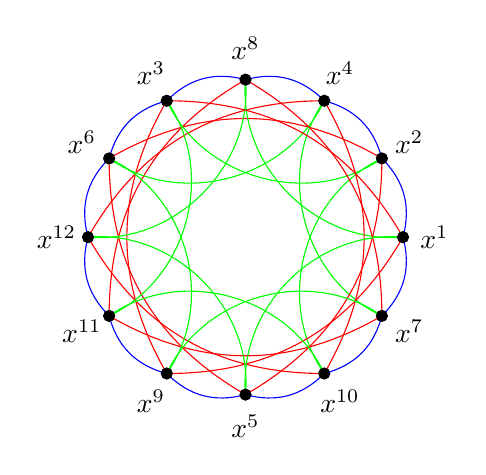
\begin{tikzpicture}
      \def\crater{12}
      \def\jumpa{-8}
      \def\jumpb{9}
      \def\diam{2cm}

      \foreach \i in {1,...,\crater} {
        \draw[blue] (360/\crater*\i : \diam) to[bend right] (360/\crater*\i+360/\crater : \diam);
        \draw[red] (360/\crater*\i : \diam) to[bend right] (360/\crater*\i+\jumpa*360/\crater : \diam);
        \draw[green] (360/\crater*\i : \diam) to[bend right=50] (360/\crater*\i+\jumpb*360/\crater : \diam);
      }
      \foreach \i in {1,...,\crater} {
        \pgfmathparse{int(mod(2^\i,13))}
        \let\exp\pgfmathresult
        \draw[fill] (360/\crater*\i: \diam) circle (2pt) +(360/\crater*\i: 0.4) node{$x^{\exp}$};
      }
    \end{tikzpicture}
    \caption{Undirected Schreier graph on $〈x〉\setminus\{1\}$ where $x^{13} = x$,
			acted upon by $(ℤ/13ℤ)^*$, generated by $S=\{2,3,5\}$ (resp.
      blue, red and green edges).}
    \label{fig:cayley}
  \end{minipage}
\end{figure}

\section{Key exchange from isogeny graphs}
\label{sec:keyex}

We would like to instantiate the key exchange protocol of
Algorithm~\ref{alg:HHS-DH} with the principal homogeneous space
$X = \Ell_q(\O)$ for the group $G = \Cl(\O)$, 
for some well chosen order $\O$ in a quadratic imaginary field. 
However, given a generic element of $\Cl(\O)$, 
the best algorithm~\cite{jao+soukharev10} to evaluate
its action on $\Ell_q(\O)$ has subexponential complexity in $q$,
making the protocol infeasible. 
The solution,
following Couveignes~\cite{cryptoeprint:2006:291},
is to fix a set $S$ of small prime ideals in $\O$,
whose action on $X$ can be computed efficiently,
and such that compositions of elements of $S$
cover the whole of $G$.
The action of an arbitrary element of $G$
is then the composition of a series of actions by small elements in $S$.
As Rostovtsev and Stolbunov~\cite{rostovtsev+stolbunov06} observed,
it is useful to visualise this decomposed action
as a walk in an isogeny graph.


\subsection{Walks in isogeny graphs}

Let $G$ be a group,
$X$ a principal homogeneous space for $G$,
and~$S$ a subset of~$G$.
The Schreier graph $\Graph(G,S,X)$
is the labelled directed graph whose vertex set is~$X$, 
and where an edge labelled by $s∈S$
links $x_1$ to $x_2$ if and only if $s\cdot x_1 = x_2$.
It is isomorphic to a Cayley graph for $G$.
If $S$ is symmetric (that is, $S^{-1}=S$), 
then we associate the same label to $s$ and $s^{-1}$, 
making the graph undirected.

A \emph{walk} in $\Graph(G,S,X)$ is a finite sequence
$(s_1,\ldots,s_n)$ of \emph{steps} in $S$. 
We define the action of this walk on $X$ as
\[
    (s_1,\ldots,s_n)·x 
    = 
    \big(\prod_{i=1}^n s_i\big)·x.
\]
In our situation $G$ is abelian,
so the order of the steps $s_i$ does not matter.
We can use this action directly in the key exchange protocol
of Algorithm~\ref{alg:HHS-DH},
by simply replacing private keys with walks instead of elements in $G$.

\begin{example}
Figure~\ref{fig:cayley}
shows $\Graph(G,S,X)$ where $G=(ℤ/13ℤ)^*$, 
%$S=T∪T^{-1}$ where $T=\{2,3,5\}$, 
$S = \{2,3,5\}\cup\{2^{-1},3^{-1},5^{-1}\}$,
and $X = \langle{x}\rangle\setminus\{1\}$ 
is a cyclic group of order $13$, minus its identity element.
The action of $G$ on $X$ is exponentiation: $g·x=x^g$.
The action of $11$, which takes $x^k$ to $x^{11k}$,
can be expressed using the walks 
$(2,5,5)$,
or $(2^{-1},3^{-1})$,
or $(3,5)$,
for example.  Note that $5$ has order $4$ modulo
$13$, thus partitioning $〈x〉\setminus\{1\}$ into $3$ cycles of
length $4$.
\end{example}

Returning to the world of isogenies,
we now take
\begin{itemize}
    \item $X=\Ell_q(\O)$ as the vertex set, for some well-chosen $q$ and $\O$;
        in particular we require $\O$ to be the maximal order (see Section~\ref{sec:sec}).
    \item $G=\Cl(\O)$ as the group acting on $X$;
    \item $S$ a set of small Elkies primes in $\O$.
        %ideals of the form $(π-λ,ℓ)$, where $ℓ$ is an
        %  Elkies prime for the isogeny class $\Ell_q(\O)$,
        %  and $λ$ is an eigenvalue of Frobenius on $E[ℓ]$. 
        %  % (i.e.\ an integer in $ℤ/ℓℤ$).
\end{itemize}
The graph $\Graph(G,S,X)$ is thus an isogeny graph, 
composed of many isogeny cycles (one for the norm of each prime in $S$) 
superimposed on the vertex set $\Ell_q(\O)$.
It is connected if $S$ generates $\Cl(\O)$.
Walks in $\Graph(G,S,X)$ are called \emph{isogeny walks}.

We compute the action of
an ideal $\frak s$ (a single \emph{isogeny step})
on an $x∈\Ell_q(\O)$ 
by choosing a representative curve $E$ with $x = j(E)$,
and computing an isogeny $ϕ_{\frak s}:E→E'$ from $E$
corresponding to $\frak{s}$;
the resulting vertex is $\frak s \cdot x = j(E')$.
The action of an isogeny walk $(\frak s_i)_i$
is then evaluated as the sequence of isogeny steps $ϕ_{\frak s_i}$. 
Algorithms for these operations are given in the next subsection. 

Using this ``smooth'' representation of elements
in $\Cl(\O)$ as isogeny walks
lets us avoid computing $\Cl(\O)$ and $\Ell_q(\O)$,
and avoid explicit ideal class arithmetic;
only isogenies between elliptic curves are computed.
In practice, we re-use the elliptic curve $E'$ from one step
as the $E$ in the next;
but we emphasize that
when isogeny walks are used for Diffie--Hellman,
the resulting public keys and shared secrets
are not the final elliptic curves,
but their $j$-invariants.


\subsection{Computing isogeny walks}

Since $\Cl(\O)$ is commutative,
we can break isogeny walks down into a succession of walks
corresponding to powers of single primes $\frak{s} = (\ell,\pi-\lambda)$;
that is, repeated applications of the isogenies $\phi_{\frak{s}}$.
Depending on $\frak{s}$,
we will compute each sequence of $\phi_{\frak s}$
using one of two different methods:
\begin{itemize}
    \item Algorithm~\ref{alg:ElkiesWalk} (\algstyle{ElkiesWalk})
        uses Algorithm~\ref{alg:ElkiesFirstStep}
        (\algstyle{ElkiesFirstStep})
        followed by a sequence of calls to Algorithm~\ref{alg:ElkiesNextStep} 
        (\algstyle{ElkiesNextStep}),
        both which use the \emph{modular polynomial} $\Phi_\ell(X, Y)$.
        This approach works for any $\frak s$.
    \item
        Algorithm~\ref{alg:VéluWalk} (\algstyle{VéluWalk})
        uses a sequence of calls to 
        Algorithm~\ref{alg:VéluStep} (\algstyle{VéluStep}).
        This approach uses \emph{torsion points} on $E$, 
        and can only be applied when
	    $\lambda$ satisfies certain properties.
\end{itemize}

Rostovtsev and Stolbunov only used analogues of 
Algorithms~\ref{alg:ElkiesFirstStep} and~\ref{alg:ElkiesNextStep}.
%which is a classical algorithm.  %% <- BS: not _that_ classical...
The introduction of Algorithm~\algstyle{VéluStep}, 
% very different in spirit from Algorithm~\algstyle{ElkiesStep} and
inspired by the SIDH cryptosystem and related protocols,
speeds up the protocol by a considerable factor;
this is the main practical contribution of our work. 
\algstyle{VéluStep} is also a key ingredient in the CSIDH protocol~\cite{csidh}.

Let us now delve into
the details of these two~\algstyle{Step} algorithms.

\begin{algorithm}
	\caption{\algstyle{ElkiesFirstStep}}
	\label{alg:ElkiesFirstStep}
	\Input{%
        $E\in\Ell_q(\O)$; 
        $(\ell,\lambda)$ defining an ideal $\frak s = (\pi-\lambda,\ell)$
    }
	\Output{$j(\frak s\cdot E)$}
    %
	$P\gets \Phi_\ell(X, j(E))$ 
    \;
    %
    \label{line:roots}
    $\{j_1, j_2\} \gets \algstyle{Roots}(P,\F_q)$ 
    \;
	%$K\gets$ Kernel of the $\ell$-isogeny from $E$ to some $E_1$ with $j(E_1) = j_1$ \label{line:kernel}\;
    \label{line:kernel}
    $K\gets \algstyle{KernelPolynomial}(\algstyle{Isogeny}(E,j_1,\ell))$ 
    \tcp*{e.g.~BMSS algorithm}
    %
	$Q\gets$ a nonzero point in $K$ %\;
    \tcp*{i.e. $(x,y)\in E(\F_q[x,y]/(y^2-f_E(x),K(x)))$}
    %
	\uIf{$\pi(Q) = [\lambda]Q$}{%
        \Return{$j_1$} \label{line:direction}
        \;
    }
	\Else{%
        \Return{$j_2$} \label{line:end_direction}
    }
\end{algorithm}

\begin{algorithm}
	\caption{\algstyle{ElkiesNextStep}}
	\label{alg:ElkiesNextStep}
    \Input{%
        $(\ell,\lambda)$ defining an ideal $\frak{s} = (\ell,\pi-\lambda)$;
        $(j_0,j_1) = (j(E),j(\frak{s}\cdot E))$ for some $E$ in $\Ell_q(\O)$
    }
    %(\ell,\lambda)$ defining an ideal $\frak s = (\pi-\lambda,\ell)$; $j_{k-1} = j(\frak s^{k-1}\cdot E)$ and $j_k = j(\frak s^{k}\cdot E)$ for some $E\in\Ell_q(\O)$ and $k\geq 1$}
    \Output{$j(\frak{s}\cdot\frak{s}\cdot E)$}
    %
    \label{alg:ElkiesNextStep:step}
	$P\gets \Phi_\ell(X, j_1) / (X - j_0)$ 
    \;
    %
	$j_2\gets$ the unique root of $P$ in $\F_q$ 
    \;
    %
	\Return{$j_2$}
    \;
\end{algorithm}

\begin{algorithm}
	\caption{\algstyle{ElkiesWalk}}
	\label{alg:ElkiesWalk}
	\Input{%
        $E\in \Ell_q(\O)$;
        $(\ell,\lambda)$ defining an ideal $\frak s = (\pi - \lambda,\ell)$;
        $k\geq 1$
    }
	\Output{$\frak s^k \cdot E$}
	$j_0 \gets j(E)$ \;
    $j_1 \gets \algstyle{ElkiesFirstStep}(E, (\ell,\lambda))$ \;
	\For{$2\leq i \leq k$}{
        $(j_0, j_1) \gets (j_1, \algstyle{ElkiesNextStep}((\ell,\lambda),(j_0,j_1)))$ 
        \;
	}
    $E_R \gets \algstyle{EllipticCurveFromJInvariant}(j_1)$ 
    \;
    %$E_R \gets$ an elliptic curve with $j$-invariant $j_1$ and order $C$ 
    \label{line:twist}
    \uIf{$\algstyle{CheckTrace}(E_R,t)$}{
        \Return{$E_R$}
        \;
    }
    \Else{
        \Return{$\algstyle{QuadraticTwist}(E_R)$}
        \;
    }
\end{algorithm}

\begin{algorithm}
	\caption{\algstyle{VéluStep}}
	\label{alg:VéluStep}
	\Input{%
        $E\in\Ell_q(\O)$; 
        $(\ell,\lambda)$ defining an ideal $\frak s = (\pi-\lambda,\ell)$;
        $r > 0$;
        $C_r = \#E(\F_{q^r})$
    }
	\Output{$\frak s\cdot E$}
    %
	\Repeat{$Q \neq 0_E$}{
        $P\gets \algstyle{Random}(E(\F_{q^r}))$ 
        \;
		$Q\gets [C_r/\ell] P$ \label{line:scalarmult}
        \;
	}
    $K\gets \prod_{i=0}^{(\ell-1)/2}(X - x([i]Q))$
    \tcp*{Kernel polynomial of isogeny} %Subgroup of order $\ell$ generated by $Q$ \;
    %
    $E_R\gets \algstyle{IsogenyFromKernel}(E,K)$ \label{line:quotient}
    \tcp*{Apply Vélu's formul\ae} %\;
    %
	\Return{$E_R$}
    \;
\end{algorithm}

\begin{algorithm}
	\caption{\algstyle{VéluWalk}}
	\label{alg:VéluWalk}
	\Input{%
        $E\in \Ell_q(\O)$;
        $(\ell,\lambda)$ defining an ideal $\frak s = (\ell,\pi - \lambda)$; 
        $k\geq 1$
    }
	\Output{$\frak s^k \cdot E$}
    %
    $r\gets \algstyle{Order}(\lambda,\ell)$ % Multiplicative order of $\lambda$ in $\Z/\ell\Z$ 
    \tcp*{Precompute and store for each $(\ell,\lambda)$}
    % \;
	$C_r \gets \# E(\F_{q^r})$ \label{line:card}
    \tcp*{Precompute and store for each $r$} 
    % \;
    \For{$1 \le i \le k$}{
        $E \gets \algstyle{VeluStep}(E,(\ell,\lambda),r,C_r)$
        \;
    }
    \Return{$E$}
\end{algorithm}

\paragraph{Elkies steps.}
Algorithms~\ref{alg:ElkiesFirstStep}
and~\ref{alg:ElkiesNextStep} 
compute single steps in the $\ell$-isogeny graph.
Their correctness
follows from the definition of the modular polynomial $\Phi_\ell$:
a cyclic $\ell$-isogeny exists between two elliptic
curves $E$ and $E'$ if and only if $\Phi_\ell(j(E), j(E')) = 0$
(see~\cite[\S6]{schoof95} and~\cite[\S3]{Elkies98} for the relevant theory).
One may use the classical modular polynomials here,
or alternative, lower-degree modular polynomials
(Atkin polynomials, for example)
with minimal adaptation to the algorithms.
In practice, $\Phi_\ell$ is precomputed and stored:
several publicly available databases exist (see~\cite{Echidna}, for example).

Given a $j$-invariant $j(E)$,
we can compute its two neighbours in the $\ell$-isogeny graph
by evaluating $P(X) = \Phi_\ell(j(E),X)$
(a polynomial of degree $\ell+1$),
and then computing its two roots in $\F_q$.
Using a Cantor--Zassenhaus-type algorithm,
this costs
$\softO(\ell\log q)$ $\F_q$-operations.

We need to make sure we move to the neighbour in the correct direction.
If we have already made one such step then this is easy:
it suffices to avoid backtracking.
Algorithm~\ref{alg:ElkiesNextStep} (\algstyle{ElkiesNextStep})
does this by
removing the factor corresponding to the previous $j$-invariant 
in Line~\ref{alg:ElkiesNextStep:step};
this algorithm can be used for all but the first of the steps
corresponding to $\frak{s}$.

In the first of many steps for $\frak{s}$,
we must choose the right direction.
Algorithm~\ref{alg:ElkiesFirstStep}
takes the two candidates,
chooses one arbitrarily,
and computes its kernel explicitly.
This costs $\softO(\ell)$ $\F_q$-operations
using the Bostan--Morain--Salvy--Schost algorithm~\cite{BMSS08}
with asymptotically fast polynomial arithmetic.
Given the polynomial defining the kernel,
we compute an element $Q$ of $\ker\phi_\frak{s}$
over an extension of $\F_q$ of degree at most $\frac{\ell-1}{2}$,
then evaluate $\pi(Q)$ and compare with $[\lambda]Q$.
If this matches, then we have chosen the right direction;
otherwise we take the other root of $P(X)$.
%This is also the critical
%part of Algorithm~\ref{alg:ElkiesNextStep}.

Algorithm~\ref{alg:ElkiesWalk} (\algstyle{ElkiesWalk}) 
combines these algorithms
to compute the iterated action of $\frak{s}$
(at Line~\ref{line:twist}, if the curve does not have correct order,
then its quadratic twist does).
Both \algstyle{ElkiesFirstStep} and \algstyle{ElkiesFirstStep}
cost $\softO(\ell\log q)$ field operations,
with the dominant step in each being the calculation of the roots of $P(X)$.
% and grows quasi-linearly with $\ell$.


\paragraph{Vélu steps.}

For some primes $\frak{s} = (\ell,\pi-\lambda)$,
we can completely avoid modular polynomials,
and the costly computation of their roots,
by constructing $\ker\phi_{\frak{s}}$ directly from $\ell$-torsion points.
Let $r$ be the order of $\lambda$ modulo $\ell$;
then $\ker\phi_{\frak s} \subseteq E(\F_{q^r})$.
If $r$ is not a multiple of the order of the other eigenvalue $\mu$
of $\pi$ on $E[\ell]$,
then $E[\ell](\F_{q^r}) = \ker\phi_{\frak s}$.
Algorithm~\ref{alg:VéluStep} (\algstyle{VéluStep}) 
exploits this fact to construct a generator $Q$ of $\ker\phi_{\frak s}$
by computing a point of order $\ell$ in $E(\F_{q^r})$.
The roots of the kernel polynomial of $\phi_{\frak s}$
are then $x(Q), \ldots, x([(\ell-1)/2]Q)$.
%Notice that the values
%of $r$ and $C_r$ could be made part of the public parameters, but we
%leave them here for clarity.

Constructing a point $Q$ of order $\ell$ in $E(\F_{q^r})$
is straightforward:
we take random points and multiply by the cofactor $C_r/\ell$,
where $C_r := \#E(\F_{q^r})$.
Each trial succeeds with probability $1 - 1/\ell$.
Note that $C_r$ can be easily (pre)computed from the Frobenius trace $t$:
if we write $C_r = q - t_r + 1$ for 
$r > 0$ (so $t_1 = t$) and $t_0 = 2$,
then the $t_r$ satisfy the standard recurrence
$t_r = t\cdot t_{r-1} - q\cdot t_{r-2}$. 

Computing the quotient curve at Line~\ref{line:quotient} is easily done
with Vélu's formulas~\cite{Velu71} using $O(\ell)$ operations in $\F_q$.
Since $\log C_r\simeq r\log q$, provided $\ell = O(\log q)$,
the costly step in Algorithm~\ref{alg:VéluStep} is the scalar
multiplication at Line~\ref{line:scalarmult}, which costs
$\softO(r^2\log q)$ $\F_q$-operations.

\paragraph{Comparing the costs.}
To summarize:
\begin{itemize}
\item Elkies steps cost $\softO(\ell\log q)$ $\F_q$-operations;
\item Vélu steps cost $\softO(r^2\log q)$ $\F_q$-operations,
    where $r$ is the order of $\lambda$ in $\Z/\ell\Z$.
\end{itemize}
In general $r = O(\ell)$, so Elkies steps should be preferred. 
However, when $r$ is particularly small
(and not a multiple of the order of the other eigenvalue),
a factor of $\ell$ can be saved using Vélu steps.
The value of $r$ directly depends on $\lambda$, which is in turn determined by
$\#E(\F_p)$ mod $\ell$. Thus, we see that better \algstyle{Step} performances
depend on the ability to find elliptic curves whose order
satisfies congruence conditions modulo small primes.
Unfortunately, we can only achieve this partially
(see Section~\ref{sec:initcurve}), so the most efficient solution is
to use Vélu steps when we can, and Elkies steps for some other primes.

In practice, Algorithm~\ref{alg:VéluStep} can be improved
by using elliptic curve models with more efficient arithmetic;
we use Montgomery arithmetic here~\cite{Montgomery87,CostelloSmith2017},
without computing $y$-coordinates. This model also
offers convenient Vélu formulas~\cite{Renes2018}.
On the other hand, the Weierstrass model is classical and universal, 
and is usually the considered model in the literature
about isogeny computations.
Hence, if the initial curve $E_0$ admits a Montgomery model, one can
compute the Vélu steps \emph{first} using Montgomery models,
and switch to Weierstrass models afterwards. Note that
we can also avoid computing $y$-coordinates in
Algorithm~\ref{alg:ElkiesFirstStep}
at Line~\ref{line:direction} if $\lambda\neq\pm\mu$.
% In this case, choosing the correct quadratic twist at
% Line~\ref{line:end_direction} is not an issue.
%% BS: I think it's best (and safer) to always ensure we're on the right twist.

\begin{remark}
    \label{rem:twist-trick}
    Note that when $r = 1$ (hence $\lambda = 1$), which is the best case
    in Algorithm~\ref{alg:VéluStep}, Vélu steps cannot be used in direction $\mu$
    using the algorithm as written above. However, switching to the quadratic
    twist of $E$ changes the sign of the Frobenius eigenvalues; 
    for instance, if $p \equiv -1\pmod{\ell}$ and $\lambda = 1$, then $\mu=-1$ and
    Vélu steps can be used in both directions with $r=1$.
    In Algorithm~\ref{alg:VéluStep}, only the curve order
    and the random point sampling need to be modified when using quadratic twists.
\end{remark}

\subsection{Sampling isogeny walks and key exchange}

We now describe precisely how one samples secret keys and performs a key
exchange in our protocol. 
Since the cost of the various isogeny walks depends on the ideals
chosen,
we will use adapted, or \emph{skewed}, 
smooth representations when sampling elements in $\Cl(\O)$
in order to minimize the total computational cost of a key exchange.

The generating set $S$ will consist of

\begin{enumerate}
\item \label{case:elkstep} Ideals $(\pi - \lambda, \ell)$ and their inverses $(\pi - \mu, \ell)$
	for very small Elkies primes $\ell$, when \emph{neither} $\lambda$ nor $\mu$
	are eligible to Vélu steps. We encode them as 
	a list $S_E$ of tuples $(\ell, \lambda, \mu)$, the \emph{Elkies part} of $S$.
\item \label{case:velustep-sym} Ideals $(\pi - \lambda, \ell)$ and their inverses $(\pi - \mu, \ell)$
	for small Elkies primes $\ell$, when \emph{both} $\lambda$ and $\mu$
	are eligible to Vélu steps. We encode them as
	a list $S_{V, 2}$ of tuples $(\ell, \lambda, \mu)$, the \emph{symmetric Vélu part} of $S$.
\item \label{case:velustep-asym} Ideals $(\pi - \lambda, \ell)$, \emph{without their inverses},
	if $\ell$ is a small Elkies prime and \emph{only} eigenvalue $\lambda$
	is eligible to Vélu steps. We encode them as a list
	$S_{V, 1}$ of tuples $(\ell, \lambda)$, the \emph{asymmetric Vélu part} of $S$.
\end{enumerate}

Looking back at Figure~\ref{fig:cycle}, in cases~\ref{case:elkstep} and~\ref{case:velustep-sym}
both directions $\lambda,\mu$ are used, while in case~\ref{case:velustep-asym} only $\lambda$ is
available.

Recall that (ephemeral) secret keys are walks in the isogeny graph.
Since the class group $\Cl(\O)$ is commutative, such a walk is fully
determined by an \emph{exponent vector}, with one exponent for each ideal in $S$
up to inverse: for an ideal $\frak s\in S$, this exponent can be negative if
$\frak s^{-1}$ also appears in $S$, and must be nonnegative otherwise.

In order to minimize the cost of computing an isogeny walk, we use a
\emph{walk length bound} for each ideal, as follows.
For each prime $\ell$ appearing in $S$, we define a bound $M_\ell$
on (the absolute value of) the exponent of ideals of norm $\ell$. As a rule,
$M_\ell$ will be much bigger in the Vélu case.
Algorithm~\algstyle{KeyGen} that generates a secret key is now
easily described (Algorithm~\ref{alg:isogeny-KeyGen}).

\begin{algorithm}
    \caption{\algstyle{KeyGen} for cryptosystems in the isogeny graph on
    $\Ell_q(\O)$ with walks based on $S$}
    \label{alg:isogeny-KeyGen}
    \Input{%
        The set $S$ given as $S_E, S_{V,2}, S_{V,1}$;
        the walk length bounds $(M_\ell)_{\ell\in S}$
    }
    \Output{A secret key $(k_\ell)_{\ell\in S}$}
    \For{$(\ell, \lambda, \mu)\in S_E\cup S_{V, 2}$} {
        $k_\ell\gets \algstyle{Random}([-M_\ell, M_\ell])$ 
        \;
    }
    \For{$(\ell, \lambda)\in S_{V, 1}$}{%
        $k_\ell\gets \algstyle{Random}([0,M_\ell])$ 
        \;
    }
    \Return{$(k_\ell)$}
\end{algorithm}

%Then, an isogeny walk is simply a sequence of isogeny
%steps, using either Elkies or Vélu steps as appropriate:
%see Algorithm~\ref{alg:walk}. 
%Algorithm~\ref{alg:keyex}
%then rephrases the generic Diffie--Hellman algorithm~\ref{alg:HHS-DH}
%in our particular setting, making explicit all public parameters involved in the
%protocol.

Algorithm~\ref{alg:isogeny-DH}
completes a Diffie--Hellman key exchange
by applying a combination of Elkies and Vélu walks
(Algorithms~\ref{alg:ElkiesWalk} and~\ref{alg:VéluWalk}, respectively).

\begin{algorithm}
    \caption{\algstyle{DH} for the isogeny graph on $\Ell_q(\O)$
        with primes in $S$}
    \label{alg:isogeny-DH}
    \Input{%
        A private key \((k_\ell)_\ell\)
        corresponding to a walk $(\frak{s}_1,\ldots,\frak{s}_n)$;
        a public key $j_B = j(E_B)$ for $E_B \in \Ell_q(O)$
    }
    \Output{%
        A shared secret $j(\prod_{i=1}^n\frak{s_i}\cdot E_B)$
    }
    %
    $E \gets \algstyle{EllipticCurveFromjInvariant}(j_B)$
    \;
    %
    \If{\textbf{not} $\algstyle{CheckTrace}(E,t)$}{%
        $E \gets \algstyle{QuadraticTwist}(E)$
        \;
    }
    \For{$(\ell,\lambda,\mu) \in S_E$}{
        \lIf{$k_\ell \ge 0$}{%
            $\nu \gets \lambda$
        }
        \lElse{%
            $\nu \gets \mu$
        }
        $E \gets \algstyle{ElkiesWalk}(E,(\ell,\nu),|k_\ell|)$
    }
    \For{$(\ell,\lambda,\mu) \in S_{V,2}$}{
        \lIf{$k_\ell \ge 0$}{%
            $\nu \gets \lambda$
        }
        \lElse{%
            $\nu \gets \mu$
        }
        $E \gets \algstyle{VéluWalk}(E,(\ell,\nu),|k_\ell|)$
        \;
    }
    \For{$(\ell,\lambda) \in S_{V,1}$}{
        $E \gets \algstyle{VéluWalk}(E,(\ell,\lambda),k_\ell)$
        \;
    }
    \Return{$j(E)$}
\end{algorithm}

%\begin{algorithm}
%	\caption{\algstyle{Walk}: an isogeny walk}
%	\label{alg:walk}
%	\Input{
%		\begin{itemize}
%		\itemsep0em
%		\item An exponent vector $k = (k_\ell)$
%		\item An initial $j$-invariant $j_I$
%		\item The set $S$ given as $S_E,\ S_{V,2},\ S_{V,1}$
%		\item The order $C$ of the public elliptic curve
%		\end{itemize}
%	}
%	$E \gets $ a curve of $j$-invariant $j_I$\;
%	\For{$(\ell, \lambda, \mu)\in S_E$}{
%		\lIf{$k_\ell\geq 1$}{
%			$E\gets \algstyle{ElkiesWalk}(E, C, \ell, \lambda, k_\ell)$
%		}
%		\lElseIf{$k_\ell\leq -1$}{
%			$E\gets \algstyle{ElkiesWalk}(E, C, \ell, \mu, |k_\ell|)$
%		}
%	}
%	\For{$(\ell, \lambda, \mu)\in S_{V,2}$}{
%		\If{$k_\ell\geq 0$}{
%			\lFor{$1\leq j \leq k_\ell$}{$E\gets \algstyle{VéluStep}(E, \ell, \lambda)$}
%		}
%		\Else{
%			\lFor{$1\leq j \leq |k_\ell|$}{$E\gets \algstyle{VéluStep}(E, \ell, \mu)$}
%		}
%	}
%	\For{$(\ell,\lambda)\in S_{V,1}$}{
%		\lFor{$1\leq j \leq k_\ell$}{$E\gets \algstyle{VéluStep}(E, \ell, \lambda)$}
%	}
%	\Return{$j(E)$}
%\end{algorithm}

%\begin{algorithm}
%  \caption{Key exchange from an isogeny graph}
%  \label{alg:keyex}
%  \Params{
%		\begin{itemize}
%		\itemsep0em
%		\item A prime power $q$ 
%		\item An ordinary elliptic curve $E_0/\F_q$ with order $C$, and maximal endomorphism ring
%		\item The set $S$ given as $S_E,\ S_{V,2},\ S_{V,1}$
%		\item Walk length bounds $M_\ell$
%		\end{itemize}
%	}
%  \Alice{
%    \Samples $k_A = \algstyle{KeySample}(S, (M_\ell))$\;
%    \Sends $j_A = \algstyle{Walk}(k_A, j(E_0), S, C)$ to Bob}
%  \Bob{
%    \Samples $k_B = \algstyle{KeySample}(S, (M_\ell))$\;
%    \Sends $j_B = \algstyle{Walk}(k_B, j(E_0), S, C)$ to Alice}
%  \Key{$j_F = \algstyle{Walk}(k_A, j_B, S, C) = \algstyle{Walk}(k_B, j_A, S, C)$}
%\end{algorithm}

\section{Public parameter selection}
\label{sec:initcurve}

It is now evident that the choice of public parameters, especially
the initial curve $E_0$, has heavy impact on the execution time:
smaller Elkies primes,
and smaller multiplicative orders of the Frobenius eigenvalues, will
lead to better practical performances. Since all of this information
is contained in the value of $\# E(\F_q)$, we now face the problem
of constructing ordinary elliptic curves with prescribed
order, or more precisely with prescribed order \emph{modulo small
primes}. Unfortunately, and in contrast with the case of
supersingular curves, no polynomial-time method to achieve this 
is known in general; the CM method~\cite{AtkinMorain93,Sutherland2012},
which solves this problem
when the corresponding class groups are small, is useless in our
setting as we will see in Section~\ref{sec:sec}.

In this section, we describe how to use the Schoof--Elkies--Atkin (SEA) point counting
algorithm with early abort, combined with the use of certain modular curves,
to construct curves whose cardinality satisfies some constraints
modulo small prime.
This is faster than choosing curves at random and computing their cardinalities
completely until a convenient one is found, but still does not allow us
to use the full power of Algorithm~\algstyle{VéluStep}.

\paragraph{Early-abort SEA.}
The SEA algorithm~\cite{schoof95,Morain95}
is a polynomial-time algorithm for
point counting on elliptic curves over a finite field. In order to compute
$N = \# E(\F_p)$, it computes the value of $N$ modulo a series
of small primes $\ell$, before combining the results via the CRT
to get the true value of $N$.
Cryptographers are usually interested in generating elliptic curves of
prime or nearly prime order. In this case, we use an \emph{early-abort}
mechanism: as soon as we detect $N \equiv 0\pmod{\ell}$ for some $\ell$, the algorithm is aborted
and a new curve is chosen.

Here, the situation is the opposite: we \emph{want} elliptic curves
whose cardinality has many small prime divisors.
To fix ideas, we choose the 512-bit prime
\[
    p = 7 \left(\prod_{2\leq\ell\leq 380,\ \ell \text{ prime}} \ell\right) - 1
\]
Then, according to section~\ref{sec:keyex}, Algorithm~\algstyle{VéluStep} can be used
for $\ell$-isogenies with $r=1$ in both directions if and only if
$N := \# E(\F_p)$ satisfies $N \equiv0\pmod{\ell}$.
We now proceed as follows:
\begin{itemize}
\item Choose a smoothness bound $B$ (we used $B = 13$).
\item Pick elliptic curves $E$ at random in $\F_p$, and use the SEA algorithm,
aborting when any $\ell\leq B$ 
with $\#E(\F_p) \not\equiv 0\pmod{\ell}$ is found.
\item For each curve which passed the tests above, complete the SEA
algorithm and estimate the key exchange running time using this
curve as a public parameter (see Section~\ref{sec:exp}).
\end{itemize}
The ``fastest'' curves now give promising candidates for $\#E(\F_p)$.

Considering the efficiency of this procedure, it is important to remark
that very few curves will pass the early-abort tests. The bound $B$ is
chosen to balance the overall cost of the first few tests with that of
the complete SEA algorithm for the curves which pass them. Therefore,
its value is somewhat implementation-dependent. In practice, one also
incorporates the test of existence of a Montgomery model for the
elliptic curve as in~\cite{OKS00}.

\paragraph{Finding the maximal order.}
Once such a curve $E_1$ has been computed, it is important to find a curve
$E_0$ having the same number of points, but whose endomorphism ring is maximal, and
to ensure that its discriminant is a large integer. Therefore, we attempt to
factor the discriminant $Δ_\pi$ of $\Z[\pi]$: if it is squarefree,
then $E_1$ already has maximal endomorphism ring, and in general the square
factors of $Δ_\pi$ indicate which isogeny volcanoes have to be climbed up
in order to find $E_0$.

\begin{remark}
    Factoring random 512-bit integers is not hard, and quadratic discriminants
    tend to be slightly smoother than random integers
    (it took less then one hour of GMP-ECM on 10 cores 
    to factor the 512-bit discriminant given at the end of this section).
    %todo: which hardware ?
    A conservative strategy would be to discard any discriminant 
    that cannot be completely factored,
    but ultimately undetected large prime-square factors
    do not present a security issue
    because computing the possible corresponding large-degree isogenies 
    is intractable (see Section~\ref{sec:sec}).
\end{remark}

\paragraph{Using the modular curve $X_1(N)$.}
Since we are looking for curves with smooth cardinalities, another
improvement to this procedure is available: instead of choosing elliptic
curves uniformly at random, we pick random candidates using
an equation for the modular curve $X_1(N)$~\cite{sutherland2012constructing},
which guarantees the existence of a rational $N$-torsion point
on the sampled elliptic curve.
This idea is used
in the procedure of selecting elliptic curves in the Elliptic Curve Method
for factoring~\cite{ECM20,GMP-ECM}.
In our implementation, we used $N = 17$. 

\paragraph{Results.}
We implemented this search using the Sage computer algebra system.
Our experiments were conducted on several machines running
Intel Xeon E5520 processors at 2.27GHz. %todo: more details
After 17,000 hours of CPU time, we found the Montgomery elliptic curve 
$
	E : y^2 = x^3 + A x^2 + x
$
over $\F_p$ with $p$ as above, and
\[
\begin{aligned}
A =\ 
& 1086133850464928038385995014077294700770364640837283 \\
& 1934324660566888732797778932142488253565145603672591 \\
& 944602210571423767689240032829444439469242521864171\,.
\end{aligned}
\]
The trace of Frobenius $t$ of $E$ is
\[
\begin{aligned}
-&147189550172528104900422131912266898599 \\
&387555512924231762107728432541952979290\,.
\end{aligned}
\]
%% p := 7*&*PrimesInInterval(2,380) - 1;
%% A := 10861338504649280383859950140772947007703646408372831934324660566888732797778932142488253565145603672591944602210571423767689240032829444439469242521864171 ;

This curve, or its twist, has a rational $\ell$-torsion point 
for each $\ell$ in
\[
  \{3, 5, 7, 11, 13, 17, 103, 523, 821, 947, 1723\}
  \,;
\]
each of these primes is Elkies.
Furthermore, $\End(E)$ is the maximal order, and its discriminant is
a 511-bit integer that has the following prime factorization:
\[
\begin{aligned}
& \scriptstyle -2^3 \cdot 20507 \cdot 67429 \cdot 11718238170290677 \cdot 12248034502305872059 \\
& \scriptstyle \cdot 60884358188204745129468762751254728712569\\
& \scriptstyle \cdot 68495197685926430905162211241300486171895491480444062860794276603493\,.
\end{aligned}
\]

Other proposals for public parameters are given in~\cite{memoire}.
In the sequel, we will argue that using this curve brings a 128-bit security level
in the classical as well as quantum setting, and we give running times of the whole
scheme in our implementation.

\section{Security}
\label{sec:sec}

We now address the security of the CRS primitive, and derived
protocols. Intuitively, these systems rely on two assumptions:
\begin{enumerate}
\item Given two elliptic curves $E,E'$ in $\Ell_q(\O)$, it is hard to
  find a (smooth degree) isogeny $ϕ:E→E'$;
\item The distribution on $\Ell_q(\O)$ induced by the random walks
  sampled in Algorithm~\ref{alg:isogeny-KeyGen} is computationally
  undistinguishable from the uniform distribution.
\end{enumerate}

We start by reviewing the known attacks for the first problem, both in
the classical and the quantum setting. Then, we formalize security
assumptions and give security proofs against passive adversaries.
Finally, we discuss key validation and protection against active
adversaries.

\subsection{Classical attacks}
\label{sec:classical-attacks}

We start by addressing the following, more general, problem:

\begin{problem}
\label{prob:isog}
  Given two ordinary elliptic curves $E,E'$ defined over a finite
  field $\F_q$, such that $\#E(\F_q)=\#E'(\F_q)$, find an isogeny walk
  $(ϕ_i)_{1≤i≤n}$ such that $ϕ_n∘\cdots∘ϕ_1(E)=E'$.
\end{problem}

This problem was studied for some time before the emergence of
isogeny-based cryptography~\cite{Gal,GHS,galbraith+stolbunov11},
because of its applications to elliptic curve
cryptography~\cite{GHS,teske06,jao+miller+venkatesan09}.  The
algorithm with the best asymptotic complexity is due to Galbraith,
Hess and Smart~\cite{GHS}. It consists of three stages:
\begin{description}
\item[Stage 0.] Use walks of \emph{ascending} isogenies to reduce to the case where
  $\End(E)\cong\End(E')$ is the maximal order.
\item[Stage 1.] Start two random walks of horizontal isogenies 
  from $E$ and $E'$; detect the
  moment when they collide using a Pollard-rho type of algorithm.
\item[Stage 2.] Reduce the size of the obtained walk using
  index-calculus techniques.
\end{description}

To understand Stage~0, recall that all isogenous elliptic curves have
the same order, and thus the same trace $t$ of the Frobenius
endomorphism $π$. Define the Frobenius discriminant $Δ_π=t^2-4q$, then
$\End(E)$ is contained in the ring of integers $\O_K$ of
$K=ℚ(\sqrt{Δ_π})$. Write $Δ_π=d^2Δ_K$, where $Δ_K$ is the
discriminant\footnote{$Δ_K$ is also called a \emph{fundamental
    discriminant}; it is in $\{0,1\}\bmod 4$, and either $Δ_K$ or
  $Δ_K/4$ is squarefree.} of $\O_K$, then for any $ℓ\mid d$ the
$ℓ$-isogeny graph of $E$ contains \emph{ascending} and
\emph{descending} isogenies and is sometimes referred to as a
\emph{volcano}~\cite{fouquet+morain02} (see Figure~\ref{fig:volcano}).
Ascending isogenies go from curves with smaller endomorphism rings to
curves with larger ones, and take us to a curve with $\End(E)≃\O_K$ in
$O(\log d)$ steps; they can be computed efficiently using the
algorithms
of~\cite{kohel,fouquet+morain02,ionica+joux13,defeo2016explicit},
thus, Stage~0 can be accomplished\footnote{This statement is assuming
  that all prime factors of $d$ are in $O(\log q)$, which is typically
  the case for isogeny-based protocols: no counter-example
	has ever been constructed.}  in time polynomial in
$\log q$.

\begin{figure}
  \centering
  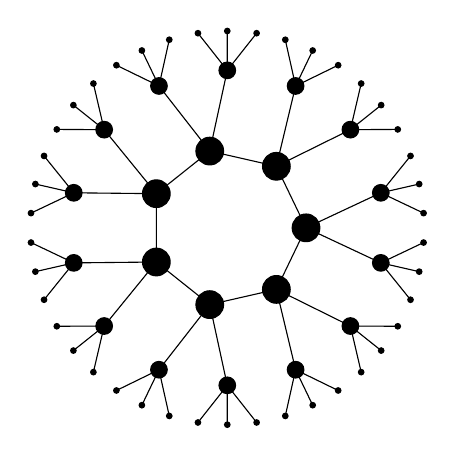
\begin{tikzpicture}
    \def\crater{7}
    \foreach \i in {1,...,\crater} {
      \draw[fill] (360/\crater*\i:1cm) circle (5pt);
      \draw (360/\crater*\i : 1cm) -- (360/\crater*\i+360/\crater : 1cm);
      \foreach \j in {-1,1} {
        \draw[fill] (360/\crater*\i : 1cm) -- (360/\crater*\i + \j*360/\crater/4 : 2cm) circle (3pt);
        \foreach \k in {-1,0,1} {
          \draw[fill] (360/\crater*\i + \j*360/\crater/4 : 2cm) --
          (360/\crater*\i + + \j*360/\crater/4 + \k*360/\crater/6 : 2.5cm) circle (1pt);
        }
      }
    }
  \end{tikzpicture}
  \caption{$3$-isogeny graph (\emph{volcano}) containing the curve
    with $j(E)=607$ over $\F_{6007}$. A larger vertex denotes a larger
    endomorphism ring.}
  \label{fig:volcano}
\end{figure}

The class $\Ell_q(\O_K)$ is the smallest among all classes
$\Ell_q(\O)$ for $\O⊂\O_K$, so it is always interesting to
reduce to it. This justifies using curves with maximal endomorphism
ring in the definition of the protocol in
Section~\ref{sec:keyex}. We remark that when $Δ_π$ is square-free, $ℤ[π]$
is the maximal order, and hence this condition is automatically satisfied.

The collision search in Stage~1 relies on the birthday paradox, thus
it has a complexity of $O(\sqrt{h(\O_K)})$, where $h(\O_K)=\#\Ell_q(\O_K)$ is the
class number of $\O_K$.  It is known that, on average,
$h(\O_K)≈0.461\cdots\sqrt{|Δ_K|}$ (see~\cite[5.10]{Cohen1993}), and,
assuming the extended Riemann hypothesis, we even have a lower bound
(see~\cite{littlewood1928class})
\[h(\O_K) ≥ 0.147\cdots\frac{(1+o(1))\sqrt{|Δ_K|}}{\log\log|Δ|}.\]
Since $Δ_K\sim q$, we expect Stage~1 to take time $O(q^{1/4})$,
thus justifying the choice of a $q$ four times as large as the
security parameter.  Unfortunately, class numbers are notoriously
difficult to compute, the current record being
for a discriminant of 300 bits~\cite{10.1007/978-3-642-14081-5_15}.
Computing the class
number for a discriminant of ${\sim 500}$ bits seems to be expensive,
albeit feasible; thus, we will only rely on these heuristic arguments
to justify the security of our proposed parameters.
% todo: check this is really the latest record

Finally, Stage~2,
which outputs an isogeny walk of size polynomial in $\log q$,
has a complexity bounded by that of Stage~1.
It therefore has no impact on our security estimates.

\begin{remark}
  The Cohen--Lenstra heuristic~\cite{10.1007/BFb0099440} predicts that
  the odd part of $\Cl(\O_K)$ is cyclic with overwhelming
  probability, and other heuristics~\cite{10.1007/3-540-44448-3_18}
  indicate that $h(\O_K)$ is likely to have a large prime factor.
  However, since there is no known way in which the group structure of
  $\Cl(\O_K)$ can affect the security of our protocol, we can 
  disregard this matter. No link between the group structure
	of $E(\F_q)$ itself and the security is known, either.
\end{remark}

\subsection{Quantum attacks}
\label{sec:quantum-attacks}

On a quantum computer, an attack with better asymptotic complexity is
given in~\cite{childs2014constructing}. It consists of two algorithms:
\begin{enumerate}
\item A (classical) algorithm that takes as input an elliptic curve
  $E∈\Ell_q(\O)$ and an ideal $\frak a∈\Cl(\O)$, and outputs the curve
  $\frak a·E$;
\item A generic quantum algorithm for the dihedral hidden subgroup
  problem (dHSP), based upon previous work of Kuperberg~\cite{Kup} and
  Regev~\cite{regev04}.
\end{enumerate}

The ideal evaluation algorithm has sub-exponential complexity
$L_q(\frac{1}{2},\frac{\sqrt{3}}{2})$.  The dHSP algorithm uses the
ideal evaluation algorithm as a (quantum) black box, the number of
queries depending on the variant:
\begin{itemize}
\item Kuperberg's algorithm uses $O(2^{\sqrt{\log q}})$ queries, and a
  storage of $O(2^{\sqrt{\log q}})$ qubits;
\item Regev's algorithm has worse query complexity, using
  $L_q(\frac{1}{2},1)$ calls to the black box, but only requires a
  storage of $\poly(\log q)$ qubits.
\end{itemize}

Based on these estimates, we expect the bit size of $q$ to grow at
worst like the square of the security parameter. However, given that
the constants implied in the complexities are not made explicit, it is
hard to estimate the impact of this attack at concrete security levels
such as those required by NIST~\cite{NIST2016}. Nevertheless, we
remark that the weaker version of Kuperberg's algorithm described
in~\cite[§2.1]{regev04}, requires about $2^{\sqrt{8\log q}}$ queries
to the black box; this number can be taken as a very conservative
lower bound, given that the described algorithm is specific to
$h(O_K)=2^n$, and also because Regev's algorithm, with its polynomial
storage requirement, is a much more realistic candidate to run on a
real world quantum computer. By taking into account the fact that each
black box query runs a quantum circuit of subexponential size itself,
we estimate that the lower bound on the number of quantum gates is at
least the square of the lower bound on the number of quantum
queries. Based on these observations, we propose in
Table~\ref{tab:sizes} parameter sizes matching three of the NIST
categories~\cite{NIST2016}.
According to this table, the public parameters we proposed
in Section~\ref{sec:initcurve} fit in NIST category~2.

\begin{table}
    \renewcommand{\arraystretch}{1.4}
    \centering
    \begin{tabular}{c@{\;}|@{\;}c@{\;}|@{\;}c@{\;}|@{\;}c@{\;}|@{\;}c@{\;}|@{\;}c}
        $\log Δ_K$ & $\log h(\O_K)$
        & \parbox{10ex}{\centering classical security}
        & \parbox{10ex}{\centering quantum queries}
        & \parbox{10ex}{\centering quantum security}
        & \parbox{10ex}{\centering NIST category}\\
        \hline
        $512$  & $256$ & $2^{128}$ & $> 2^{64}$ & $2^{128}$ & 2\\
        $768$  & $384$ & $2^{192}$ & $> 2^{78}$ & $> 2^{156}$ & 3\\
        $1024$ & $512$ & $2^{256}$ & $> 2^{90}$ & $> 2^{180}$ & 5
        \\
        \hline
    \end{tabular}
    \smallskip
    \caption{Suggested parameter sizes at different security levels.}
    \label{tab:sizes}
\end{table}

\subsection{Security proofs}
\label{sec:proofs}

We now formalize the assumptions needed to prove the security of the
key exchange protocol, and other derived protocols such as PKEs and
KEMs, in various models. Given the similarity with the classical
Diffie--Hellman protocol on a cyclic group, our assumptions are
mostly modeled on those used in that context. Here we are
essentially following the lead of
Couveignes~\cite{cryptoeprint:2006:291} and
Stolbunov~\cite{Stol,Stolbunov2012}.
However, we take their analyses a
step further by explicitly modeling the hardness of distinguishing
random walks on Cayley graphs from the uniform distribution: this
yields stronger proofs and a better separation of security concerns.

We will write $x\rand{σ} X$ for an element taken from a set $X$
according to a probability distribution $σ$. If $X$ is finite,
then we write $x\uni X$ for an element taken according to the uniform
distribution.

For the rest of this section $q$ is a prime power, $\O$ is an order in
a quadratic imaginary field with discriminant $Δ\sim q$, $\Cl(\O)$ is
the class group of $\O$, $\Ell_q(\O)$ is the (non-empty) set of
elliptic curves with complex multiplication by $\O$, and $E_0$ is a
fixed curve in $\Ell_q(\O)$. Finally, $S$ is a set of ideals of $\O$
with norm polynomial in $\log q$, and $σ$ is a probability
distribution on $S^*$, used to sample secrets in the key exchange
protocol.

The assumption needed to prove security of the protocols is 
the hardness of a problem analogous to 
the classic Decisional Diffie--Hellman (DDH) problem.

\begin{definition}[Isogeny Walk DDH (IW-DDH)]
    Given a triplet of curves $(E_a,E_b,E_{ab})$
    sampled with probability $\frac{1}{2}$ 
    from one of the following two distributions
  \begin{align*}
    \mathcal{R}_{q,Δ,σ} &= \left\{\bigl((\frak a_i)_i·E_0,(\frak b_i)_i·E_0,E'\bigr) \suchthat
                        (\frak a_i)_i,(\frak b_i)_i\rand{σ}S^*,\;
                        E'\uni\Ell_q(\O)\right\},\\
    \mathcal{W}_{q,Δ,σ} &= \left\{\bigl((\frak a_i)_i·E_0,(\frak b_i)_i·E_0,(\frak a_i)·(\frak b_i)·E_0\bigr) \suchthat
                          (\frak a_i)_i,(\frak b_i)_i\rand{σ}S^*\right\},
  \end{align*}
  decide from which of the two they were sampled.
\end{definition}

We split this problem into two finer-grained problems. 
The first is that of distinguishing between 
commutative squares sampled uniformly at random 
and commutative squares sampled from the distribution $σ$.

\begin{definition}[Isogeny Walk Distinguishing (IWD)]
    Given a triplet of curves $(E_a,E_b,E_{ab})$
    sampled with probability $\frac{1}{2}$ 
    from one of the following two distributions
  \begin{align*}
    \mathcal{G}_{q,Δ} &= \left\{(\frak a·E_0,\frak b·E_0,\frak{ab}·E_0) \suchthat
                        \frak a,\frak b\uni\Cl(\O)\right\},\\
    \mathcal{W}_{q,Δ,σ} &= \left\{\bigl((\frak a_i)_i·E_0,(\frak b_i)_i·E_0,(\frak a_i)·(\frak b_i)·E_0\bigr) \suchthat
                          (\frak a_i)_i,(\frak b_i)_i\rand{σ}S^*\right\},
  \end{align*}
  decide from which of the two they were sampled.
\end{definition}

The second problem is a group-action analogue of DDH.
It also appears in~\cite{cryptoeprint:2006:291} under the
name \emph{vectorization}, and in~\cite{Stol,Stolbunov2012} under the
name DDHAP.
 
\begin{definition}[Class Group Action DDH (CGA-DDH)]
    Given a triplet of curves $(E_a,E_b,E_{ab})$
    sampled with probability $\frac{1}{2}$ 
    from one of the following two distributions
  \begin{align*}
    \mathcal{U}_{q,Δ} &= \left\{(E_a,E_b,E_{ab}) \suchthat E_a,E_b,E_{ab}\uni\Ell_q(\O)\right\},\\
    \mathcal{G}_{q,Δ} &= \left\{(\frak a·E_0,\frak b·E_0,\frak{ab}·E_0) \suchthat
                        \frak a,\frak b\uni\Cl(\O)\right\},
  \end{align*}
  decide from which of the two they were sampled.
\end{definition}

We want to prove the security of protocols based on the primitive of
Section~\ref{sec:keyex} under the CGA-DDH and IWD assumptions
combined. To do this we give a lemma showing that CGA-DDH and IWD
together imply IW-DDH. The technique is straightforward: we use an
IW-DDH oracle to solve both the CGA-DDH and IWD problems, showing that
at least one of the two must be solvable with non-negligible
advantage. The only technical difficulty lies in the fact that we need
an efficient way to simulate the uniform distribution on $\Ell_q(\O)$;
for this, we use another Cayley graph on $\Ell_q(\O)$, potentially
with a larger edge set, that is proven
in~\cite{jao+miller+venkatesan09} to be an expander.

We let $\Adv[A]{IW-DDH}$ be the \emph{advantage} of an adversary $A$
against IW-DDH, defined as the probability that $A$ answers correctly,
minus $\frac{1}{2}$:
\[2\Adv[A]{IW-DDH} = \Proba\bigl[A(\mathcal{R}_{q,Δ,σ}) = 1\bigr] -
  \Proba\bigl[A(\mathcal{W}_{q,Δ,σ}) = 1\bigr].\] %
We define $\Adv[A]{CGA-DDH}$ and $\Adv[A]{IWD}$ similarly. By switching
answers if needed, we can assume all advantages are positive.
We let $\Adv{xxx}(t)$ denote the maximum of $\Adv[A]{xxx}$ over all
adversaries using at most $t$ resources (e.g.\ running time, queries,
etc.).

\begin{lemma}
\label{lem:adv}
  Assuming GRH, for $q$ large enough and for any bound $t$ on running
  time, and for any $\epsilon>0$,
  \[\Adv{IW-DDH}(t) ≤ 2\Adv{IWD}(t+\poly(\log q, \log\epsilon)) + \Adv{CGA-DDH}(t) + \epsilon.\]
\end{lemma}
\begin{proof}[Sketch]
  We start with an adversary $A$ for IW-DDH, and we construct two simulators
  $S$ and $T$ for CGA-DDH and IWD respectively.

  The simulator $S$ simply passes its inputs to $A$,
  and returns $A$'s response.

  The simulator $T$ receives a triplet $(E_a,E_b,E_{ab})$ taken from
  $\mathcal{G}_{q,Δ}$ or $\mathcal{W}_{q,Δ,σ}$. It flips a coin
  to decide which of the two following actions it will do:
  \begin{itemize}
  \item It forwards $(E_a,E_b,E_{ab})$ to $A$, and returns the same bit
    as given by $A$;
  \item It generates a random curve $E_c∈\Ell_q(\O)$, forwards
    $(E_a,E_b,E_c)$ to $A$, and returns the opposite bit to the one
    given by $A$.
  \end{itemize}
  
  The curve $E_c$ must be taken from a distribution close to uniform
  for the simulator to work. The only way at our disposal to sample
  $E_c$ uniformly would be to sample a uniform $\frak c∈\O$, and take
  $E_c=\frak c·E_0$, but this would be too costly. Instead we
  use~\cite[Theorem~1.5]{jao+miller+venkatesan09},
	combined with standard results about random walks in
	expander graphs (for instance, an easy adaptation of the proof
	of~\cite[Lemma~2.1]{jao+miller+venkatesan09}), to sample $E_c$ so
  that any curve in $\Ell_q(\O)$ is taken with probability between
  % todo: Jean, you mentioned that you could get closer to the uniform
  % distribution by lengthening the walks?
  $(1-\epsilon)/h(\O)$ and $(1+\epsilon)/h(\O)$,
	using only $\poly(\log q, \log\epsilon)$ operations.
	We can consider this sampling as follows:
	with probability $1-\epsilon$, sample $E_c$ \emph{uniformly},
	and with probability $\epsilon$ sample it from
	an unknown probability distribution.

  Now, if $T$ forwarded $(E_a,E_b,E_{ab})$ untouched, then we immediately get
    \begin{align*}
        2\Adv[T]{IWD} 
        & = 
        \Adv[A]{IW-DDH} - \Adv[S]{CGA-DDH}
        \,
        \intertext{while if $T$ forwarded $(E_a,E_b,E_c)$, then we get}
        2\Adv[T]{IWD} 
        & \geq 
        \Adv[A]{IW-DDH} - (1-\epsilon)\Adv[S]{CGA-DDH} - \epsilon
        \,.
    \end{align*}
  Averaging over the two outcomes concludes the proof.
    \qed
\end{proof}

Finally, we define an analogue of the classic 
Computational Diffie--Hellman (CDH) problem for groups.
Using the same techniques as above, we can prove the
security of the relevant protocols based only on CGA-CDH and IWD,
\emph{without} the generalized Riemann hypothesis.

\begin{definition}[Class Group Action CDH (CGA-CDH)]
  Given curves $E_a=\frak a·E_0$ and $E_b=\frak b·E_0$, with
  $\frak a,\frak b\uni\Cl(\O)$, compute the curve
  $E_{ab}=\frak{ab}·E_0$.
\end{definition}

We can now prove the security of our schemes. Stolbunov already proved
the security of HHS Diffie--Hellman under the equivalent of CGA-DDH~\cite{Stol}.
By repeating the same steps, we can prove the following theorem.

\begin{theorem}
    If the CGA-DDH and IWD assumptions hold, assuming GRH, 
    the key-agreement protocol defined by 
    Algorithms~\ref{alg:isogeny-KeyGen} and~\ref{alg:isogeny-DH}
    is session-key secure in the authenticated-links adversarial model 
    of Canetti and Krawczyk~\cite{canetti}.
\end{theorem}

Similarly, we can prove the IND-CPA security of the hashed El Gamal
protocol derived from Algorithm~\ref{alg:isogeny-KeyGen} by replicating the
classical techniques of, for
instance,~\cite[20.4.11]{galbraith2012mathematics}.

\begin{theorem}
    Assuming CGA-CDH and IWD, the hashed El Gamal protocol derived from
    Algorithms~\ref{alg:isogeny-KeyGen} and~\ref{alg:isogeny-DH}
    is IND-CPA secure in the random oracle model.
\end{theorem}


\paragraph{A heuristic discussion of the IWD assumption.}

From its very definition, the IWD problem depends on
the probability distribution $σ$ we use to sample
random walks in the isogeny graph. In this paragraph,
we provide heuristic arguments suggesting that 
the IWD instances generated by Algorithm~\ref{alg:isogeny-DH} are hard,
provided
\begin{enumerate}
    \item the keyspace size is at least $\sqrt{|Δ_K|}$, and
    \item $S$ is \emph{not too small}, i.e. the number of
        isogeny degrees used is in $\Omega(\log q)$.
\end{enumerate}

At present, proving rapid mixing of random walks with such
parameters seems out of reach, even under number-theoretic
hypotheses such as GRH. The best results available,
like~\cite[Theorem~1.5]{jao+miller+venkatesan09}
(which we used in the proof of Lemma~\ref{lem:adv}),
typically require isogeny degrees in $\Omega((\log q)^B)$
for some $B>2$, and fully random walks that are not,
for example, skewed towards smaller-degree isogenies.

However, numerical evidence suggests that
these theoretical results are too weak. In~\cite[7.2]{jao+miller+venkatesan09},
it is asked whether an analogue of the previous theorem would
be true with the sole constraint $B>1$. In~\cite[Section~3]{GHS},
it is mentioned that many fewer split primes are needed to walk
in the isogeny graph than theoretically expected.
Practical evidence also suggests that the rapid mixing
properties are not lost with skewed random walks:
such walks are used in~\cite{galbraith+stolbunov11},
to accelerate an algorithm solving Problem~\ref{prob:isog}.
We believe that these experiments can bring some evidence
in favor of relying on the IWD assumptions with more aggressive
parameters than those provided by GRH.


\subsection{Key validation and active security}

Modern practice in cryptography mandates the use of stronger security
notions than IND-CPA.  From the DLP assumption, it is easy to
construct protocols with strong security against active adversaries.
For example, it is well known that the hashed El Gamal KEM achieves
IND-CCA security in the random oracle model under various
assumptions~\cite[§7]{10.1007/3-540-45353-9_12,cryptoeprint:1999:007,doi:10.1137/S0097539702403773}.

All of these constructions crucially rely on \emph{key validation}, 
i.e.\ Alice must verify that the public data sent by Bob defines valid
protocol data (e.g., valid elements of a cyclic group), or abort if
this is not the case.
Failure to perform key validation may result in catastrophic attacks,
such as small subgroup~\cite{10.1007/BFb0052240}, invalid
point~\cite{10.1007/3-540-44598-6_8}, and invalid curve
attacks~\cite{Ciet2005}.  

In our context, key validation amounts to
verifying that the curve sent by Bob really is an element of
$\Ell_q(\O_K)$. Failure to do so exposes Alice to an \emph{invalid
  graph attack}, where Bob forces Alice onto an isogeny class with much
smaller discriminant, or different Elkies primes, and learns something
on Alice's secret.

Fortunately, key validation is relatively easy for protocols based on
the CRS primitive. All we need to check is that the received curve has
the right order, and has maximal endomorphism ring. Notice that,
because these algorithms only operate on public data, they do not need
to be constant-time.

\paragraph{Verifying the curve order.} Since we already know the trace $t$
of the Frobenius endomorphism of all curves in $\Ell_q(\O)$, 
we only need to check that the given $E$ has order $q+1-t$.
Assuming that $E$ is cyclic, or contains a
cyclic group of order larger than $4\sqrt{q}$, a very efficient
randomized algorithm consists in taking a random point $P$ and
verifying that it has the expected order.  This task is easy if the
factorization of $q+1-t$ is known.

Concretely, the curve given in Section~\ref{sec:initcurve} has order
\[N = 2^2 · 3^2 · 5 · 7 · 11 · 13^2 · 17 · 103 · 523 · 821 ·
  1174286389 · m,\] %
where $m$ is a $432$-bit prime, and its group structure is
$ℤ/2ℤ×ℤ/\frac{N}{2}ℤ$. To check that a curve is in the same isogeny
class, we repeatedly take random points until we find one with order
$N/2$.

\paragraph{Verifying the endomorphism ring level.} 
The curve order verification proves that $\End(E)$ 
is contained between $ℤ[π]$ and $\O_K$. 
We have already seen that there is only a finite number of
possible rings: their indices in $\O_K$ must divide $d$ where $d^2=Δ_π/Δ_K$.
Ascending and descending isogenies connect curves with different endomorphism
rings, thus we are left with the problem of verifying that $E$ is on
the crater of any $ℓ$-volcano for $ℓ\mid d$.

Assuming that no large prime divides $d$, this check can be
accomplished efficiently by performing random walks in the volcanoes,
as described in~\cite[\S4.2]{kohel} or~\cite{fouquet+morain02}. 
Note that if we choose $Δ_π$ square-free, 
then the only possible endomorphism ring is $\O_K$,
and there is nothing to be done.

Concretely, for the curve of Section~\ref{sec:initcurve}
we have $Δ_π/Δ_K=2^2$,
so there are exactly two possible endomorphism rings. Looking at
the action of the Frobenius endomorphism, we see that $\End(E)=\O_K$
if and only if $E[2]≃(ℤ/2ℤ)^2$.

\begin{example}
    Let $p$ and $\O$ be as in Section~\ref{sec:initcurve}.
    Suppose we are given the value
    \begin{align*}
        \alpha & = 
        6774653762400376370473362072511594555277819004969905295950079
        \\
        & \quad\ 
        3811735672493775187377489138828163987156950866238907910693817
        \\
        & \quad\ 
        71311397884649111333755665289025
    \end{align*}
    in $\F_p$.  It is claimed that $\alpha$ is in $\Ell_p(\O)$;
    that is, it is a valid public key for the system with parameters
    defined in Section~\ref{sec:initcurve}.
    Following the discussion above,
    to validate $\alpha$ as a public key,
    it suffices to exhibit a curve with $j$-invariant $\alpha$,
    full rational $2$-torsion,
    and a point of order $N/2$.
    Using standard formul\ae{},
    we find that the two $\F_p$-isomorphism classes of elliptic curves
    with $j$-invariant $\alpha$
    are represented by the Montgomery curve
    $E_\alpha/\F_p: y^2 = x(x^2 + Ax + 1)$
    with
    \begin{align*}
        A & = 
        4193809979435365668528368375333535083388979993941154941880421
        \\
        & \quad\ 
        8343694887415884661259992796948986954858364460542381754613120
        \\
        & \quad\ 
        78403116671641017301728201394907
    \end{align*}
    and its quadratic twist, $E_\alpha'$.
    Checking the $2$-torsion first,
    we have $E_\alpha[2](\F_p) \cong E_\alpha'[2](\F_p) \cong (\Z/2\Z)^2$,
    because $A^2 - 4$ is a square in $\F_p$.
    Trying points on $E_\alpha$,
    we find that $(23,\sqrt{23(23^2 + 23A + 1)})$ in $E_\alpha(\F_p)$
    has exact order $N/2$.
    We conclude that $\End(E_\alpha) = \O$,
    so $\alpha$ is a valid public key.
    (In fact, $E_\alpha$ is connected to the initial curve
    by a single $3$-isogeny step.)
\end{example}

\paragraph{Consequences for cryptographic constructions.}
Since both of the checks above can be done much more efficiently 
than evaluating a single isogeny walk, 
we conclude that key validation is not only possible,
but highly efficient for protocols based on the CRS construction. 
This stands in stark contrast to the case of SIDH,
where key validation is known to be
problematic~\cite{galbraithsecurity}, and even conjectured to be has
hard as breaking the system~\cite{cryptoeprint:2018:336}.

Thanks to this efficient key validation, 
we can obtain CCA-secure encryption from the
CRS action without resorting to generic transforms such as
Fujisaki--Okamoto~\cite{10.1007/3-540-48405-1_34}, unlike the case of
SIKE~\cite{SIKE,10.1007/978-3-319-70500-2_12}. This in turn enables
applications such as non-interactive key exchange, for which no
practical post-quantum scheme was known prior to~\cite{csidh}.


\section{Experimental results}
\label{sec:exp}

In order to demonstrate that our key-exchange protocol is usable
at standard security levels, we implemented it in the Julia
programming language.
We developed a small Julia package, built upon 
the computer algebra package Nemo~\cite{nemo},
to implement basic functionalities
for elliptic curves over finite fields~\cite{package}.
Experiments were conducted on a machine running a 3.2GHz Intel Xeon processor.
%todo: more details ?

First, consider the
time to compute one step for an ideal $\frak s = (\ell,\pi-\lambda)$.
Using \algstyle{ElkiesStep}, this is approximately
the cost of finding the roots of the modular polynomial,
which is roughly $0.017\cdot\ell$ seconds in our implementation.
Using \algstyle{VéluStep}, the cost of a step is approximately
that of one scalar multiplication in $E(\F_{q^r})$.
Table~\ref{tab:time-vs-r} lists per-step times in our implementation,
for the extension degrees relevant to our parameters.

\begin{table}
    \centering
    \begin{tabular}{r@{\;}|@{\;}c@{\ \ }c@{\ \ }c@{\ \ }c@{\ \ }c@{\ \ }c@{\ \ }c}
        $r$ & 1 & 3 & 4 & 5 & 7 & 8 & 9 \\
        \hline
        time (s) & 0.02 & 0.10 & 0.15 & 0.24 & 0.8 & 1.15 & 1.3
    \end{tabular}
    \smallskip
    \caption{Timings for computing scalar multiplications in
    $E(\F_{p^r})$, the dominant operation in \algstyle{VéluStep}
    (Algorithm~\ref{alg:VéluStep}), as a function of the extension
    degree $r$.}
    \label{tab:time-vs-r}
\end{table}

Using this data, finding efficient bounds $M_\ell$
offering a sufficient key space size is easily seen to be an
integer optimization problem. In order to find a
satisfactory solution, we used the following heuristic procedure.
Given a time bound $T$, let \algstyle{KeySpaceSize}$(T)$ be
the key space size obtained when each $M_\ell$ is the greatest such
that the \emph{total time spent on $\ell$-isogenies} is less than $T$.
Then, we look for the \emph{least $T$} such that
$
	\algstyle{KeySpaceSize}(T)\geq 2^{256}
$
according to Section~\ref{sec:sec}, using dichotomic search.
While the bounds $M_\ell$
we obtain are most likely not the best possible, intuitively
the outcome does not fall very far from the optimal.

In this way, we obtain a proposal for the bounds $M_\ell$
to be used in Algorithm~\ref{alg:isogeny-KeyGen}. Table~\ref{tab:VéluSteps}
lists the isogeny degrees amenable to Algorithm~\ref{alg:VéluStep}, with
the corresponding extension degree $r$ 
(a star denotes that the twisted curve
allows us to use both directions in the isogeny graph,
as in Remark~\ref{rem:twist-trick}).
Table~\ref{tab:ElkiesSteps}
lists other primes for which we apply Algorithm~\algstyle{ElkiesStep}.

\begin{table}
    \centering
    \begin{tabular}{l|@{\;}r@{\;}|@{\;}l@{\;}||@{\;}l|r@{\;}|@{\;}l}
        $r$ & $M_\ell$ & $\ell$
        &
        $r$ & $M_\ell$ & $\ell$
        \\
        \hline
        1* & 409 & 3, 5, 7, 11, 13, 17, 103
        &
        5 & 34 & 31, 61, 1321
        \\
        1 & 409 & 523, 821, 947, 1723
        &
        7 & 10 & 547
        \\
        3 & 81 & 19, 661
        &
        8 & 7 & 881
        \\
        4 & 54 & 1013, 1181
        &
        9 & 6 & 1693
        \\
        \hline
    \end{tabular}
    \smallskip
    \caption{Primes $\ell$ amenable to \algstyle{VéluStep}
    (Algorithm~\ref{alg:VéluStep}) for our candidate isogeny graph,
    with corresponding $r$-values and proposed walk length bounds $M_\ell$.}
    \label{tab:VéluSteps}
\end{table}

\begin{table}
    \centering
    \begin{tabular}{r@{\;}|@{\;}l@{\;}||@{\;}r@{\;}|@{\;}l@{\;}||@{\;}r@{\;}|@{\;}l@{\;}}
        $M_\ell$ & $\ell$
        &
        $M_\ell$ & $\ell$
        &
        $M_\ell$ & $\ell$
        \\
        \hline
        % line 1
        20 & 23
        &
        9  & 47
        &
        2  & 157, 163, 167, 191, 193, 197, 223, 229
        \\
        % line 2
        16 & 29
        &
        6  & 71, 73
        &
        1  & 241, 251, 257, 277, 283, 293, 307,
        \\
        % line 3
        12 & 37
        &
        5  & 89
        &
        1  & 317, 349, 359, 373, 383, 401, 421,
        \\
        % line 4
        11 & 41
        &
        4  & 107, 109, 113
        &
        1  & 431, 433, 439, 443, 449, 457, 467
        \\
        % line 5
        10 & 43
        &
        3  & 131, 151
        &
        \\
        \hline
        % line 6
    \end{tabular}
    \smallskip
    \caption{Primes $\ell$ amenable to 
        Algorithm~\ref{alg:ElkiesWalk} (\algstyle{ElkiesWalk})
        for our candidate isogeny graph, 
        with proposed walk length bounds $M_\ell$.}
    \label{tab:ElkiesSteps}
\end{table}

Using this proposal, we estimate the cost of a single walk in the
isogeny graph to be approximately 465 seconds, bringing the global
Diffie--Hellman key-exchange cost to 930 seconds (with $T = 8.2s$).
These timings are~\emph{worst-case}
in the sense that the number of isogeny steps is taken
to be exactly $M_\ell$ for each $\ell$.

We stress the fact that this implementation
is \emph{not} optimised. Besides general gains on field arithmetic,
optimised C code could easily beat our proof-of-concept implementation
on critical points of our algorithms, for instance the root finding steps 
in Algorithms~\ref{alg:ElkiesFirstStep}
and~\ref{alg:ElkiesNextStep}.

For comparison, without using Algorithm~\ref{alg:VéluStep}, the
total key-exchange time would exceed 2000 seconds:
our ideas thus bring an improvement by a factor of over 2 over the
original protocol. A longer search for efficient public
parameters would bring further improvement.

\section{Conclusion}

In this work, we demonstrated that the Couveignes-Rostovtsev-Stolbunov
framework can be improved to become practical at standard pre- and
post-quantum security levels, especially if an optimized C implementation
is made. The main obstacle to better performances is the difficulty
to generate efficient system parameters: even with lots of computational
power, one cannot expect doing \emph{only} Vélu steps. In this regard,
the CSIDH protocol~\cite{csidh}, which overcomes this problem using
supersingular curves instead of ordinary ones, is promising.

A particularly nice feature of our protocol is its key validation property,
that opens a lot of cryptographic doors. However, side-channel-resistant
implementations remain an interesting problem for future work.


\bibliographystyle{splncs04}
\bibliography{refs}

\end{document}

%  LocalWords:  Rostovtsev Stolbunov isogenies morphism isogeny
%  LocalWords:  isomorphism coprime isogenous endomorphism bijection
%  LocalWords:  Endomorphisms cryptosystem Elkies Frobenius torsor
%  LocalWords:  Couveignes isomorphisms undirected Schreier
